% =============================================================================
%  Machine Learning for Petroleum Engineers Using Python
%  Módulo 3 · Clase 4: Clasificación Multiclase --- Facies de Hugoton (SEG 2016)
%  SLB Ecuador | UDLA
%
%  Compilar: pdflatex -shell-escape presentacion.tex (x2 para refs)
% =============================================================================
\documentclass[aspectratio=169, 11pt]{beamer}

% ── Codificación y lenguaje ──────────────────────────────────────────────────
\usepackage[T1]{fontenc}
\usepackage[utf8]{inputenc}
\usepackage[spanish,es-noshorthands]{babel}

% ── Fuentes ──────────────────────────────────────────────────────────────────
\usepackage{FiraSans}
\usepackage{FiraMono}
\renewcommand{\familydefault}{\sfdefault}

% ── Gráficos y diagramas ────────────────────────────────────────────────────
\usepackage{graphicx}
\usepackage{tikz}
\usetikzlibrary{arrows.meta, positioning, shapes.geometric, calc, fit, decorations.pathreplacing}
\usepackage{fontawesome5}

% ── Código fuente ────────────────────────────────────────────────────────────
\usepackage{minted}
\usepackage{tcolorbox}
\tcbuselibrary{minted, skins, breakable}

% ── Tablas y utilidades ──────────────────────────────────────────────────────
\usepackage{amsmath}
\usepackage{colortbl}
\usepackage{booktabs}
\usepackage{multicol}
\usepackage{hyperref}
\usepackage{calc}

% =============================================================================
%  PALETA DE COLORES (rojo UDLA + variantes)
% =============================================================================
\definecolor{arcaRed}{HTML}{C82B40}
\definecolor{arcaDark}{HTML}{6B1525}
\definecolor{udlaCrimson}{HTML}{A31545}
\definecolor{arcaGray}{HTML}{F5F5F5}
\definecolor{arcaLightGray}{HTML}{EBEBEB}
\definecolor{textDark}{HTML}{2D2D2D}
\definecolor{textMuted}{HTML}{6B7280}
\definecolor{codeGreen}{HTML}{16A34A}
\definecolor{codeBlue}{HTML}{2563EB}
\definecolor{codeOrange}{HTML}{EA580C}
\definecolor{slbBlue}{HTML}{0014DC}
\definecolor{terminalBg}{HTML}{0F172A}
\definecolor{terminalGreen}{HTML}{86EFAC}
\definecolor{terminalMuted}{HTML}{94A3B8}
\definecolor{codeBg}{HTML}{FAFAFA}

% =============================================================================
%  CONFIGURACIÓN DEL TEMA BEAMER
% =============================================================================
\usetheme{default}
\usecolortheme{default}

\setbeamertemplate{navigation symbols}{}
\setbeamertemplate{footline}{}
\setbeamertemplate{headline}{}

\setbeamercolor{normal text}{fg=textDark}
\setbeamercolor{frametitle}{fg=arcaRed, bg=white}
\setbeamercolor{title}{fg=white}
\setbeamercolor{subtitle}{fg=white!85}
\setbeamercolor{author}{fg=white!80}
\setbeamercolor{date}{fg=white!70}
\setbeamercolor{item}{fg=arcaRed}
\setbeamercolor{subitem}{fg=arcaDark}
\setbeamercolor{block title}{fg=white, bg=arcaRed}
\setbeamercolor{block body}{fg=textDark, bg=arcaGray}
\setbeamercolor{block title alerted}{fg=white, bg=codeOrange}
\setbeamercolor{block body alerted}{fg=textDark, bg=arcaGray}
\setbeamercolor{block title example}{fg=white, bg=codeGreen}
\setbeamercolor{block body example}{fg=textDark, bg=arcaGray}
\setbeamercolor{section in toc}{fg=arcaDark}

\setbeamerfont{frametitle}{size=\Large, series=\bfseries}
\setbeamerfont{title}{size=\huge, series=\bfseries}
\setbeamerfont{subtitle}{size=\large}
\setbeamerfont{author}{size=\normalsize}
\setbeamerfont{date}{size=\small}
\setbeamerfont{block title}{size=\normalsize, series=\bfseries}
\setbeamerfont{footnote}{size=\tiny}

\setbeamertemplate{itemize item}{\scriptsize\raise1.5pt\hbox{\color{arcaRed}$\blacktriangleright$}}
\setbeamertemplate{itemize subitem}{\scriptsize\raise1pt\hbox{\color{arcaDark}$\bullet$}}
\setbeamertemplate{enumerate items}[default]
\setbeamercolor{enumerate item}{fg=arcaRed}

% =============================================================================
%  HEADER
% =============================================================================
\setbeamertemplate{headline}{%
  \begin{tikzpicture}[remember picture, overlay]
    \fill[arcaDark] (current page.north west) rectangle
      ([yshift=-0.7cm]current page.north east);
    \node[anchor=west, inner sep=0pt] at
      ([xshift=0.6cm, yshift=-0.35cm]current page.north west)
      {
\includegraphics[height=0.45cm]{../logo_udla_white.png}};
    \node[anchor=east, inner sep=0pt] at
      ([xshift=-0.6cm, yshift=-0.35cm]current page.north east)
      {
\includegraphics[height=0.42cm]{../SLB_white.png}};
  \end{tikzpicture}%
  \vspace{0.7cm}%
}

% =============================================================================
%  FOOTER
% =============================================================================
\setbeamertemplate{footline}{%
  \begin{tikzpicture}[remember picture, overlay]
    \draw[arcaLightGray, line width=0.4pt]
      ([yshift=0.55cm, xshift=0.6cm]current page.south west) --
      ([yshift=0.55cm, xshift=-0.6cm]current page.south east);
    \node[anchor=south, font=\tiny\color{textMuted}] at
      ([yshift=0.15cm]current page.south)
      {Machine Learning for Petroleum Engineers Using Python \(\cdot\) SLB Ecuador};
    \node[anchor=south east, font=\scriptsize\bfseries\color{arcaRed}] at
      ([xshift=-0.6cm, yshift=0.15cm]current page.south east)
      {\insertframenumber};
  \end{tikzpicture}%
}

% =============================================================================
%  FRAMETITLE personalizado con línea roja
% =============================================================================
\setbeamertemplate{frametitle}{%
  \vspace{0.25cm}%
  \usebeamerfont{frametitle}\usebeamercolor[fg]{frametitle}\insertframetitle%
  \par\vspace{2pt}%
  \begin{tikzpicture}
    \fill[arcaRed] (0,0) rectangle (3cm, 1.5pt);
    \fill[arcaLightGray] (3cm,0) rectangle (\textwidth, 0.5pt);
  \end{tikzpicture}%
  \vspace{0.1cm}%
}

% =============================================================================
%  ESTILO DE BLOQUES DE CÓDIGO (minted + tcolorbox)
% =============================================================================
\newtcblisting{pyblock}[1][]{%
  listing engine=minted,
  minted language=python,
  minted style=xcode,
  minted options={
    fontsize=\small,
    linenos=false,
    breaklines=true,
    python3=true
  },
  enhanced,
  colback=codeBg,
  colframe=arcaRed,
  left=8pt,
  right=6pt,
  top=5pt,
  bottom=5pt,
  boxrule=0pt,
  leftrule=3pt,
  arc=3pt,
  listing only,
  title={\hspace{-2pt}\faPython\hspace{5pt}Python},
  fonttitle=\scriptsize\bfseries,
  colbacktitle=arcaRed,
  coltitle=white,
  attach boxed title to top left={xshift=8pt, yshift=-7pt},
  boxed title style={
    arc=2pt, boxrule=0pt,
    top=1.5pt, bottom=1.5pt, left=6pt, right=6pt
  },
  drop fuzzy shadow=black!12,
  #1
}

\newtcblisting{outputblock}[1][]{%
  listing engine=minted,
  minted language=text,
  minted style=bw,
  minted options={
    fontsize=\small,
    breaklines=true,
    formatcom=\color{terminalGreen}
  },
  enhanced,
  colback=terminalBg,
  colframe=terminalBg,
  coltext=terminalGreen,
  left=10pt, right=6pt, top=5pt, bottom=5pt,
  boxrule=0pt,
  arc=3pt,
  listing only,
  title={\hspace{-2pt}\faTerminal\hspace{5pt}Output},
  fonttitle=\scriptsize\bfseries,
  colbacktitle=terminalGreen!85!black,
  coltitle=terminalBg,
  attach boxed title to top left={xshift=8pt, yshift=-7pt},
  boxed title style={
    arc=2pt, boxrule=0pt,
    top=1.5pt, bottom=1.5pt, left=6pt, right=6pt
  },
  #1
}

% =============================================================================
%  SECTION DIVIDERS
% =============================================================================
\newcommand{\sectionframe}[2]{%
  \begingroup
    \setbeamertemplate{headline}{}
    \setbeamertemplate{footline}{}
    \setbeamertemplate{navigation symbols}{}
    \begin{frame}[plain, noframenumbering]
      \begin{tikzpicture}[remember picture, overlay]
        \fill[arcaRed] (current page.south west) rectangle (current page.north east);
        \node[anchor=center, text=white, font=\Huge\bfseries, text width=15cm,
              align=center] at ([yshift=0.5cm]current page.center)
              {\hyphenpenalty=10000\exhyphenpenalty=10000 #1};
        \node[anchor=center, text=white!80, font=\large, text width=10cm,
              align=center] at ([yshift=-0.8cm]current page.center) {#2};
      \end{tikzpicture}
    \end{frame}
  \endgroup
}

% =============================================================================
%  METADATOS
% =============================================================================
\title{Machine Learning for Petroleum Engineers\\Using Python}
\subtitle{Módulo 3 · Clase 4: Clasificación Multiclase --- Facies de Hugoton}
\author{Carlos Enrique Mosquera Trujillo}
\date{2026}

% =============================================================================
%  DOCUMENTO
% =============================================================================
% =============================================================================
%  DOCUMENTO
% =============================================================================
\begin{document}
% ── Colores de facies (mismos de las figuras) ────────────────────────────────
\definecolor{facSS}{HTML}{EAB308}
\definecolor{facCSiS}{HTML}{D97706}
\definecolor{facFSiS}{HTML}{92400E}
\definecolor{facSiSh}{HTML}{78716C}
\definecolor{facMS}{HTML}{94A3B8}
\definecolor{facWS}{HTML}{60A5FA}
\definecolor{facD}{HTML}{C82B40}
\definecolor{facPS}{HTML}{2563EB}
\definecolor{facBS}{HTML}{1E3A8A}
\newcommand{\chip}[1]{\tikz{\fill[#1] (0,0) rectangle (0.28,0.18);}}

% ── PORTADA ──────────────────────────────────────────────────────────────────
{
\setbeamertemplate{headline}{}
\setbeamertemplate{footline}{}
\begin{frame}[plain, noframenumbering]
  \begin{tikzpicture}[remember picture, overlay]
    \fill[white] (current page.south west) rectangle (current page.north east);
    \fill[arcaRed] (current page.north west) rectangle ([yshift=-0.35cm]current page.north east);
    \fill[arcaDark] (current page.south west) rectangle ([yshift=0.35cm]current page.south east);
    \fill[arcaRed]
      ([xshift=1.1cm, yshift=-0.35cm]current page.north west) rectangle
      ([xshift=1.15cm, yshift=0.35cm]current page.south west);
    \node[anchor=north west, inner sep=0pt] at
      ([xshift=1.8cm, yshift=-1.2cm]current page.north west)
      {
\includegraphics[height=1.6cm]{../logo_udla.png}};
    \node[anchor=north east, inner sep=0pt] at
      ([xshift=-1.5cm, yshift=-1.2cm]current page.north east)
      {
\includegraphics[height=1.5cm]{../SLB.png}};
    \node[anchor=center, text=arcaDark, text width=14.5cm, align=center] at
      ([yshift=0.95cm]current page.center) {
        {\LARGE\bfseries Machine Learning for Petroleum Engineers}\\[8pt]
        {\LARGE\bfseries Using Python}
      };
    \fill[arcaRed]
      ([yshift=-0.35cm, xshift=-3.2cm]current page.center) rectangle
      ([yshift=-0.28cm, xshift=3.2cm]current page.center);
    \node[anchor=center, text=arcaRed, font=\large, text width=13cm, align=center] at
      ([yshift=-1.3cm]current page.center) {
        Módulo 3 · Clase 4\\[3pt]
        Clasificación Multiclase: el Mapa de Facies del Campo
      };
    \node[anchor=center, text=textMuted, font=\normalsize] at
      ([yshift=-2.5cm]current page.center) {
        {\color{arcaRed}\faUser}\hspace{6pt}Carlos Enrique Mosquera Trujillo
        \hspace{16pt}
        {\color{arcaRed}\faIndustry}\hspace{4pt}SLB Ecuador
      };
  \end{tikzpicture}
\end{frame}
}

% ── RECAP + RUTA ─────────────────────────────────────────────────────────────
\begin{frame}[shrink=8]{Dónde Estamos}
  \vspace{-4pt}
  \begin{columns}[T]
    \begin{column}{0.48\textwidth}
      {\small\color{arcaDark}\bfseries\faCheckCircle\hspace{5pt}Ya tenemos:}
      \vspace{4pt}
      {\footnotesize\color{textMuted}
      \begin{itemize}\setlength{\itemsep}{3pt}
        \item[{\color{codeGreen}\scriptsize\faCheck}]
          Regresión lineal: predecir un \textbf{número} (Clase 1)
        \item[{\color{codeGreen}\scriptsize\faCheck}]
          Logística: predecir \textbf{una de dos} etiquetas (Clase 2)
        \item[{\color{codeGreen}\scriptsize\faCheck}]
          Árboles y \textbf{Random Forest}: la no linealidad (Clase 3)
        \item[{\color{codeGreen}\scriptsize\faCheck}]
          El hilo de siempre: métricas + \textbf{costo de negocio}
      \end{itemize}
      }
      \vspace{6pt}
      {\scriptsize\color{textMuted}\itshape
        Pero el subsuelo casi nunca pregunta ``¿arena sí o no?''.
        Pregunta \textbf{``¿cuál de todas?''}.}
    \end{column}
    \begin{column}{0.48\textwidth}
      {\small\color{arcaDark}\bfseries\faForward\hspace{5pt}Hoy:}
      \vspace{4pt}
      {\footnotesize\color{textMuted}
      \begin{itemize}\setlength{\itemsep}{3pt}
        \item[{\color{arcaRed}\scriptsize\faArrowRight}]
          Clasificar entre \textbf{9 facies} a la vez --- un dataset nuevo:
          \textbf{Hugoton, Kansas}
        \item[{\color{arcaRed}\scriptsize\faArrowRight}]
          \textbf{Codificar} variables: el idioma que los modelos entienden
        \item[{\color{arcaRed}\scriptsize\faArrowRight}]
          Métricas multiclase: matriz \(9\times9\), macro vs weighted
        \item[{\color{arcaRed}\scriptsize\faStar}]
          El costo de negocio, ahora con \textbf{matriz de penalización}
      \end{itemize}
      }
      \vspace{4pt}
      {\scriptsize\color{arcaDark}\itshape
        Y al final, sembramos la pregunta que abre la Clase 5:
        ¿quién decide las \textbf{perillas} del modelo?}
    \end{column}
  \end{columns}
\end{frame}

% ═════════════════════════════════════════════════════════════════════════════
\sectionframe{El Problema Multiclase}{Cuando dos etiquetas no alcanzan}
% ═════════════════════════════════════════════════════════════════════════════

% ── ANDRAGOGÍA: YA CLASIFICAN EN MÁS DE DOS ──────────────────────────────────
\begin{frame}[shrink=8]{Ustedes Ya Clasifican en Más de Dos}
  \vspace{-4pt}
  {\small\color{arcaDark}\bfseries
    Piensen en la última vez que describieron ripios en el pozo o un núcleo en el laboratorio.}

  \vspace{8pt}
  \begin{columns}[T]
    \begin{column}{0.48\textwidth}
      \begin{tcolorbox}[colback=arcaGray, colframe=arcaRed, boxrule=0pt, leftrule=3pt,
        arc=3pt, left=6pt, right=6pt, top=5pt, bottom=5pt]
        {\scriptsize\color{arcaRed}\bfseries\faEye\hspace{4pt}LO QUE HACEN EN EL CAMPO}\\[4pt]
        {\scriptsize\color{textMuted}
          El geólogo de pozo no reporta ``roca sí / roca no''.
          Reporta: \textbf{arenisca}, \textbf{limolita}, \textbf{lutita},
          \textbf{caliza}, \textbf{dolomita}\ldots{} y discute los casos
          dudosos con el registro en la mano.}
      \end{tcolorbox}
      \vspace{6pt}
      {\scriptsize\color{textMuted}
        Eso es exactamente \textbf{clasificación multiclase}: elegir
        \textbf{una entre varias} categorías, para cada muestra.}
    \end{column}
    \begin{column}{0.48\textwidth}
      {\footnotesize\color{textMuted}
      \begin{itemize}\setlength{\itemsep}{5pt}
        \item[{\color{arcaRed}\scriptsize\faArrowRight}]
          En la Clase 2 lo \textbf{simplificamos} a propósito:
          ¿lutita o no lutita? Dos etiquetas.
        \item[{\color{arcaRed}\scriptsize\faArrowRight}]
          Hoy quitamos la simplificación: el modelo debe elegir
          entre \textbf{9 facies}, pie a pie.
        \item[{\color{codeGreen}\scriptsize\faCheck}]
          La buena noticia: \textbf{casi todo lo que saben se recicla} ---
          train/test, accuracy, precision, recall, el bosque.
        \item[{\color{arcaRed}\scriptsize\faExclamationTriangle}]
          Lo nuevo: cómo \textbf{alimentar} categorías al modelo
          y cómo \textbf{leer} 9 clases a la vez.
      \end{itemize}
      }
    \end{column}
  \end{columns}
\end{frame}

% ── QUÉ CAMBIA DE 2 A 9 ──────────────────────────────────────────────────────
\begin{frame}[shrink=8]{¿Qué Cambia al Pasar de 2 a 9 Clases?}
  \vspace{-4pt}
  {\small\color{arcaDark}\bfseries
    Menos de lo que temen, más de lo que parece.}

  \vspace{8pt}
  {\footnotesize
  \begin{tabular}{@{}p{4.1cm}p{4.6cm}p{4.9cm}@{}}
    \toprule
    & {\color{arcaDark}\bfseries Binario (Clase 2--3)} & {\color{arcaRed}\bfseries Multiclase (hoy)} \\
    \midrule
    El modelo responde & lutita / no lutita & \textbf{una de 9 facies} \\
    Probabilidades & una: \(P(\text{lutita})\) & \textbf{nueve}, y suman 1 \\
    Matriz de confusión & \(2\times2\): 4 casillas & \(9\times9\): \textbf{81 casillas} \\
    Precision / recall & un número de cada & \textbf{uno por clase} (9 pares) \\
    Costo de negocio & FP vs FN & \textbf{matriz de penalización} \\
    El código & \texttt{.fit()} / \texttt{.predict()} & \textbf{idéntico} \\
    \bottomrule
  \end{tabular}
  }

  \vspace{10pt}
  {\footnotesize\color{textMuted}
  \begin{itemize}\setlength{\itemsep}{3pt}
    \item[{\color{codeGreen}\scriptsize\faCheck}]
      \texttt{scikit-learn} detecta solo cuántas clases hay en \texttt{y}: el flujo no cambia.
    \item[{\color{arcaRed}\scriptsize\faArrowRight}]
      Lo que sí cambia: \textbf{preparar los datos} y \textbf{leer los resultados}.
      Ahí está la clase de hoy.
  \end{itemize}
  }
\end{frame}

% ═════════════════════════════════════════════════════════════════════════════
\sectionframe{El Dataset: Hugoton, Kansas}{La primera competencia de ML en geociencias}
% ═════════════════════════════════════════════════════════════════════════════

% ── HISTORIA ─────────────────────────────────────────────────────────────────
\begin{frame}[shrink=8]{Un Campo Gigante y una Competencia}
  \vspace{-4pt}
  {\small\color{arcaDark}\bfseries
    Hugoton (Kansas, EE.\,UU.): uno de los campos de gas más grandes de Norteamérica.}

  \vspace{8pt}
  \begin{columns}[T]
    \begin{column}{0.52\textwidth}
      {\footnotesize\color{textMuted}
      \begin{itemize}\setlength{\itemsep}{5pt}
        \item[{\color{arcaRed}\scriptsize\faIndustry}]
          Reservorio en carbonatos y areniscas del \textbf{Pérmico}
          (Grupo Council Grove): ciclos que alternan ambientes
          \textbf{marinos} y \textbf{no marinos}.
        \item[{\color{arcaRed}\scriptsize\faTrophy}]
          En 2016 la \textbf{SEG} lanzó con estos datos la primera
          competencia de \emph{machine learning} en geociencias:
          predecir \textbf{facies} desde registros.
        \item[{\color{arcaRed}\scriptsize\faUsers}]
          Cientos de equipos en el mundo compitieron con
          \textbf{estas mismas columnas} que van a usar hoy.
      \end{itemize}
      }
    \end{column}
    \begin{column}{0.44\textwidth}
      \begin{tcolorbox}[colback=arcaGray, colframe=arcaRed, boxrule=0pt, leftrule=3pt,
        arc=3pt, left=6pt, right=6pt, top=5pt, bottom=5pt]
        {\scriptsize\color{arcaDark}\bfseries\faDatabase\hspace{4pt}LA TABLA}\\[4pt]
        {\scriptsize\color{textMuted}
          \textbf{4\,149 filas} = intervalos de medio pie\\
          \textbf{10 pozos} con núcleo descrito\\
          \textbf{5 registros} + 2 variables de contexto\\
          \textbf{1 target}: la facies (9 categorías)}
      \end{tcolorbox}
      \vspace{6pt}
      {\scriptsize\color{textMuted}\itshape
        ¿Por qué existe el dataset? Describir núcleo es caro:
        solo algunos pozos lo tienen. El registro eléctrico, en cambio,
        \textbf{lo tienen todos}.}
    \end{column}
  \end{columns}
\end{frame}

% ── ACOTAR EL PROBLEMA ───────────────────────────────────────────────────────
\begin{frame}[shrink=8]{Acotar el Problema (Como Siempre, Antes de Modelar)}
  \vspace{-4pt}
  {\small\color{arcaDark}\bfseries
    La tabla que llenamos en cada clase, ahora en versión multiclase.}

  \vspace{8pt}
  {\footnotesize
  \begin{tabular}{@{}p{3.6cm}p{10.2cm}@{}}
    \toprule
    {\color{arcaDark}\bfseries Pregunta de negocio} &
      ¿Qué facies hay en cada medio pie de los pozos \textbf{sin núcleo},
      usando solo sus registros? \\
    \midrule
    {\color{arcaDark}\bfseries Target} &
      \texttt{Facies} --- 9 categorías geológicas \\
    \midrule
    {\color{arcaDark}\bfseries Features} &
      5 registros (\texttt{GR}, \texttt{ILD\_log10}, \texttt{DeltaPHI},
      \texttt{PHIND}, \texttt{PE}) + contexto (\texttt{NM\_M},
      \texttt{RELPOS}, \texttt{Formation}) \\
    \midrule
    {\color{arcaDark}\bfseries Métrica de éxito} &
      accuracy y \textbf{F1 por clase} --- y al final, la
      \textbf{penalización total} (costo multiclase) \\
    \midrule
    {\color{arcaDark}\bfseries Récord a batir} &
      el modelo tonto (siempre la facies más común):
      \textbf{23\,\% de aciertos} \\
    \bottomrule
  \end{tabular}
  }

  \vspace{8pt}
  {\scriptsize\color{textMuted}\itshape
    Regla de la casa: sin esta tabla no se escribe ni una línea de código.}
\end{frame}

% ── QUÉ ES UNA FACIES ────────────────────────────────────────────────────────
\begin{frame}[shrink=8]{Primero lo Primero: ¿Qué es una Facies?}
  \vspace{-4pt}
  {\small\color{arcaDark}\bfseries
    Antes de predecir facies, acordemos qué estamos prediciendo.}

  \vspace{8pt}
  \begin{columns}[T]
    \begin{column}{0.48\textwidth}
      \begin{tcolorbox}[colback=arcaGray, colframe=arcaRed, boxrule=0pt, leftrule=3pt,
        arc=3pt, left=6pt, right=6pt, top=5pt, bottom=5pt]
        {\scriptsize\color{arcaRed}\bfseries\faLayerGroup\hspace{4pt}LA IDEA}\\[4pt]
        {\scriptsize\color{textMuted}
          Una \textbf{facies} es un ``tipo de roca'': un paquete de
          características (grano, textura, minerales, fósiles) que
          se repiten juntas porque la roca se formó en el
          \textbf{mismo ambiente de depósito} --- una playa,
          una laguna, un arrecife.}
      \end{tcolorbox}
      \vspace{6pt}
      {\scriptsize\color{textMuted}\itshape
        Analogía: dos lotes de cemento de la misma planta y la misma
        receta se comportan igual en el pozo. Dos rocas de la misma
        facies, también.}
    \end{column}
    \begin{column}{0.48\textwidth}
      {\footnotesize\color{textMuted}
      \begin{itemize}\setlength{\itemsep}{5pt}
        \item[{\color{arcaRed}\scriptsize\faArrowRight}]
          ¿Por qué le importa al ingeniero? Porque la facies
          \textbf{controla la porosidad y la permeabilidad}:
          el mapa de facies es un mapa de \textbf{calidad de roca}.
        \item[{\color{arcaRed}\scriptsize\faArrowRight}]
          Con facies se \textbf{correlaciona} entre pozos, se decide
          \textbf{dónde completar} y se construye el modelo geológico
          del yacimiento.
        \item[{\color{codeGreen}\scriptsize\faCheck}]
          La describe un geólogo mirando el \textbf{núcleo}\ldots{}
          cuando hay núcleo. Nuestro modelo intentará hacerlo
          \textbf{desde los registros}.
      \end{itemize}
      }
    \end{column}
  \end{columns}
\end{frame}

% ── LAS 9 FACIES ─────────────────────────────────────────────────────────────
\begin{frame}[shrink=12]{Las 9 Facies: Nuestro Menú de Categorías}
  \vspace{-4pt}
  {\small\color{arcaDark}\bfseries
    Tres son de ambiente no marino, seis de ambiente marino. Guarden los colores: nos acompañan toda la clase.}

  \vspace{6pt}
  {\footnotesize
  \begin{tabular}{@{}clp{6.6cm}c@{}}
    \toprule
    & {\color{arcaDark}\bfseries Código} & {\color{arcaDark}\bfseries Qué es} & {\color{arcaDark}\bfseries Ambiente} \\
    \midrule
    \chip{facSS}   & \texttt{SS}   & Arenisca & no marino \\
    \chip{facCSiS} & \texttt{CSiS} & Limolita gruesa & no marino \\
    \chip{facFSiS} & \texttt{FSiS} & Limolita fina & no marino \\
    \chip{facSiSh} & \texttt{SiSh} & Limolita y lutita marina & marino \\
    \chip{facMS}   & \texttt{MS}   & Mudstone (caliza de grano muy fino) & marino \\
    \chip{facWS}   & \texttt{WS}   & Wackestone (caliza con matriz de lodo) & marino \\
    \chip{facD}    & \texttt{D}    & Dolomita & marino \\
    \chip{facPS}   & \texttt{PS}   & Packstone--grainstone (caliza granular) & marino \\
    \chip{facBS}   & \texttt{BS}   & Bafflestone (caliza de algas) & marino \\
    \bottomrule
  \end{tabular}
  }

  \vspace{6pt}
  {\scriptsize\color{textMuted}
  \begin{itemize}\setlength{\itemsep}{2pt}
    \item[{\color{arcaRed}\scriptsize\faArrowRight}]
      Ojo geológico: varias son \textbf{vecinas de grano}: una limolita gruesa y una fina
      se parecen \emph{muchísimo}. Recuerden esto cuando veamos los errores del modelo.
  \end{itemize}
  }
\end{frame}

% ── VARIABLES UNA A UNA ──────────────────────────────────────────────────────
\begin{frame}[shrink=12]{Las Variables, Una a Una (Lectura Física)}
  \vspace{-4pt}
  {\small\color{arcaDark}\bfseries
    Antes de dárselas al modelo, entendamos qué mide cada una.}

  \vspace{6pt}
  {\footnotesize
  \begin{tabular}{@{}llp{7.6cm}@{}}
    \toprule
    {\color{arcaDark}\bfseries Columna} & {\color{arcaDark}\bfseries Tipo} &
    {\color{arcaDark}\bfseries Qué nos dice} \\
    \midrule
    \texttt{GR} & numérica & Radioactividad natural: las \textbf{arcillas radian más} \\
    \texttt{ILD\_log10} & numérica & Resistividad profunda (en log): fluidos y litología \\
    \texttt{DeltaPHI} & numérica & Diferencia entre dos porosidades: sensible a litología \\
    \texttt{PHIND} & numérica & Porosidad promedio neutrón--densidad \\
    \texttt{PE} & numérica & Efecto fotoeléctrico: \textbf{huella de la mineralogía} \\
    \texttt{NM\_M} & \textbf{categórica} (2) & Contexto: intervalo \textbf{no marino (1) o marino (2)} \\
    \texttt{RELPOS} & numérica & Posición relativa dentro del ciclo estratigráfico (1 = tope) \\
    \texttt{Formation} & \textbf{categórica} (14) & En qué formación está la muestra (A1 SH, B5 LM, \ldots) \\
    \bottomrule
  \end{tabular}
  }

  \vspace{6pt}
  {\scriptsize\color{textMuted}
  \begin{itemize}\setlength{\itemsep}{2pt}
    \item[{\color{arcaRed}\scriptsize\faExclamationTriangle}]
      Dos columnas \textbf{no son números}: \texttt{NM\_M} y \texttt{Formation}.
      Todavía no sabemos metérselas al modelo --- ese es el tema de la próxima sección.
  \end{itemize}
  }
\end{frame}

% ── PERFIL DE POZO ───────────────────────────────────────────────────────────
\begin{frame}[shrink=8]{Así se Ve un Pozo del Dataset}
  \vspace{-4pt}
  \begin{columns}[T]
    \begin{column}{0.56\textwidth}
      \centering
      
\includegraphics[height=0.78\textheight]{fig_perfil_pozo.png}
    \end{column}
    \begin{column}{0.40\textwidth}
      {\footnotesize\color{textMuted}
      \begin{itemize}\setlength{\itemsep}{5pt}
        \item[{\color{arcaRed}\scriptsize\faArrowRight}]
          Cada medio pie tiene sus registros \textbf{y} la facies
          descrita en el núcleo (la columna de colores).
        \item[{\color{arcaRed}\scriptsize\faArrowRight}]
          Arriba domina lo \textbf{no marino} (cafés y amarillos);
          abajo, los carbonatos \textbf{marinos} (azules).
        \item[{\color{codeGreen}\scriptsize\faCheck}]
          Fíjense cómo el GR sube en las facies arcillosas y el PE
          cambia entre areniscas y calizas: \textbf{ahí hay señal}.
        \item[{\color{arcaRed}\scriptsize\faBullseye}]
          La tarea del modelo: \textbf{reconstruir la columna de
          colores} viendo solo las tres curvas.
      \end{itemize}
      }
    \end{column}
  \end{columns}
\end{frame}

% ── DESCRIBE ─────────────────────────────────────────────────────────────────
\begin{frame}[fragile,shrink=28]{Primer Vistazo con \texttt{describe()}}
  \vspace{-4pt}
  {\small\color{arcaDark}\bfseries
    Como en cada clase: números resumen primero, interpretación física al lado.}

  \vspace{4pt}
  \begin{columns}[T]
    \begin{column}{0.56\textwidth}
      \begin{pyblock}
url = "https://raw.githubusercontent.com/..."
df = pd.read_csv(url)
print(df.shape)
df[['GR','DeltaPHI','PHIND',
    'PE']].describe().round(2)
      \end{pyblock}
      \vspace{2pt}
      \begin{outputblock}
(4149, 11)
         GR  DeltaPHI  PHIND      PE
count  4149      4149   4149    3232
mean   64.9      4.40   13.2    3.73
std    30.3      5.27    7.1    0.90
min    10.2    -21.83    0.6    0.20
max   361.2     19.31   84.4    8.09
      \end{outputblock}
    \end{column}
    \begin{column}{0.40\textwidth}
      {\scriptsize\color{textMuted}
      \begin{itemize}\setlength{\itemsep}{5pt}
        \item[{\color{arcaRed}\scriptsize\faArrowRight}]
          GR máximo \textbf{361 API}: lutitas calientes,
          muy radioactivas. El promedio (65) es roca normal.
        \item[{\color{arcaRed}\scriptsize\faArrowRight}]
          \texttt{DeltaPHI} tiene \textbf{negativos}: normal,
          es una \emph{diferencia} de porosidades.
        \item[{\color{arcaRed}\scriptsize\faExclamationTriangle}]
          Miren el \texttt{count} de \texttt{PE}:
          \textbf{3\,232 de 4\,149}. Faltan casi mil valores.
          Siguiente slide.
      \end{itemize}
      }
    \end{column}
  \end{columns}
\end{frame}

% ── FALTANTES ────────────────────────────────────────────────────────────────
\begin{frame}[fragile,shrink=22]{Datos Faltantes: una Decisión, No un Accidente}
  \vspace{-4pt}
  {\small\color{arcaDark}\bfseries
    A 3 pozos no les corrieron la herramienta de PE. ¿Qué hacemos?}

  \vspace{4pt}
  \begin{columns}[T]
    \begin{column}{0.52\textwidth}
      \begin{pyblock}
print(df['PE'].isna().sum())
print(df[df['PE'].isna()]['Well Name'].unique())

df = df.dropna().reset_index(drop=True)
print(df.shape)
      \end{pyblock}
      \vspace{2pt}
      \begin{outputblock}
917
['ALEXANDER D' 'KIMZEY A' 'Recruit F9']
(3232, 11)
      \end{outputblock}
    \end{column}
    \begin{column}{0.44\textwidth}
      {\scriptsize\color{textMuted}
      \begin{itemize}\setlength{\itemsep}{4pt}
        \item[{\color{arcaRed}\scriptsize\faQuestion}]
          Opciones: \textbf{quitar las filas}, quitar la columna
          \texttt{PE}, o \textbf{inventar} el valor (imputar).
        \item[{\color{codeGreen}\scriptsize\faCheck}]
          Hoy: quitar filas. Es la opción \textbf{honesta y simple},
          y nos quedan 3\,232 muestras de 8 pozos.
        \item[{\color{arcaRed}\scriptsize\faExclamationTriangle}]
          Quitar \texttt{PE} sería tirar una de las mejores huellas
          de mineralogía --- lo comprobaremos con las importancias.
        \item[{\color{arcaRed}\scriptsize\faArrowRight}]
          ¿Y la tercera opción --- \textbf{imputar}? Rellenar el hueco
          con un valor razonable. Merece sus propias slides: van ya.
      \end{itemize}
      }
    \end{column}
  \end{columns}
\end{frame}

% ── IMPUTACIÓN: DISTRIBUCIÓN ─────────────────────────────────────────────────
\begin{frame}[shrink=14]{Imputar: Rellenar, Pero con Cabeza}
  \vspace{-6pt}
  \begin{columns}[T]
    \begin{column}{0.6\textwidth}
      \centering
      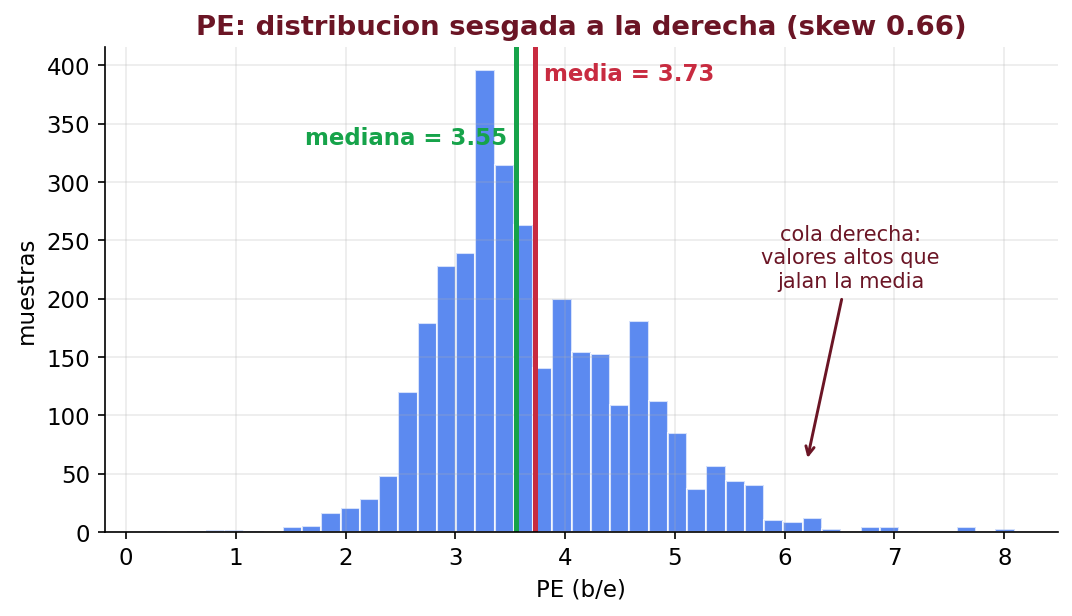
\includegraphics[width=\textwidth]{fig_pe_dist.png}
    \end{column}
    \begin{column}{0.36\textwidth}
      {\footnotesize\color{textMuted}
      \begin{itemize}\setlength{\itemsep}{5pt}
        \item[{\color{arcaRed}\scriptsize\faArrowRight}]
          Si van a inventar un valor, que sea uno \textbf{típico}.
          ¿Cuál? Depende de la \textbf{forma de la distribución}.
        \item[{\color{arcaRed}\scriptsize\faExclamationTriangle}]
          PE tiene \textbf{cola derecha}: los valores altos
          \textbf{jalan la media} hacia arriba (3.73).
          La \textbf{mediana} (3.55) no se deja arrastrar.
        \item[{\color{codeGreen}\scriptsize\faCheck}]
          Regla práctica: distribución \textbf{simétrica}
          \(\to\) media o mediana da igual;
          \textbf{sesgada o con extremos} \(\to\) \textbf{mediana}.
        \item[{\color{arcaRed}\scriptsize\faEye}]
          Caso extremo en este dataset: GR (skew 2.0 por las
          lutitas calientes). Ahí la media sí mentiría.
      \end{itemize}
      }
    \end{column}
  \end{columns}
\end{frame}

% ── IMPUTACIÓN: MENÚ DE MÉTODOS ──────────────────────────────────────────────
\begin{frame}[shrink=14]{El Menú de la Imputación: Qué Usar en Cada Caso}
  \vspace{-4pt}
  {\footnotesize
  \begin{tabular}{@{}lp{4.2cm}p{4.6cm}p{3.4cm}@{}}
    \toprule
    {\color{arcaDark}\bfseries Método} & {\color{arcaDark}\bfseries Qué hace} &
    {\color{arcaDark}\bfseries Cuándo elegirlo} & {\color{arcaDark}\bfseries Riesgo} \\
    \midrule
    Quitar filas & descarta muestras incompletas & faltan pocas filas y sobran datos
      & perder pozos o clases enteras \\
    Quitar columna & descarta la variable & la variable aporta poco
      & botar señal valiosa (¡PE!) \\
    Media & rellena con el promedio & distribución \textbf{simétrica}, faltante aleatorio
      & la arrastran los extremos \\
    Mediana & rellena con el valor central & distribución \textbf{sesgada} (como PE)
      & aplana la variabilidad \\
    Por grupo & mediana \emph{dentro} de cada formación o pozo & el grupo explica
      la variable & grupos chicos \(\to\) ruido \\
    Con modelo & predice el faltante desde las otras variables (KNN, regresión)
      & falta mucho y la variable es clave & complejidad + fugas \\
    \bottomrule
  \end{tabular}
  }

  \vspace{8pt}
  {\footnotesize\color{textMuted}
  \begin{itemize}\setlength{\itemsep}{3pt}
    \item[{\color{codeGreen}\scriptsize\faCheck}]
      Lo probamos con nuestro RF: quitar filas \textbf{0.764}, mediana \textbf{0.762},
      media \textbf{0.767}, mediana por formación \textbf{0.755}. Aquí \textbf{empatan} ---
      el faltante era ordenado (3 pozos) y PE tiene sesgo moderado.
    \item[{\color{arcaRed}\scriptsize\faExclamationTriangle}]
      Detalle fino que dejamos sembrado: la media/mediana se calcula
      \textbf{solo con el train} --- calcularla con todo es \emph{fuga de información}.
      El porqué, en la Clase 5.
  \end{itemize}
  }
\end{frame}

% ── BALANCE ──────────────────────────────────────────────────────────────────
\begin{frame}{El Balance: 9 Clases, Soportes Muy Distintos}
  \vspace{-6pt}
  \begin{columns}[T]
    \begin{column}{0.62\textwidth}
      \centering
      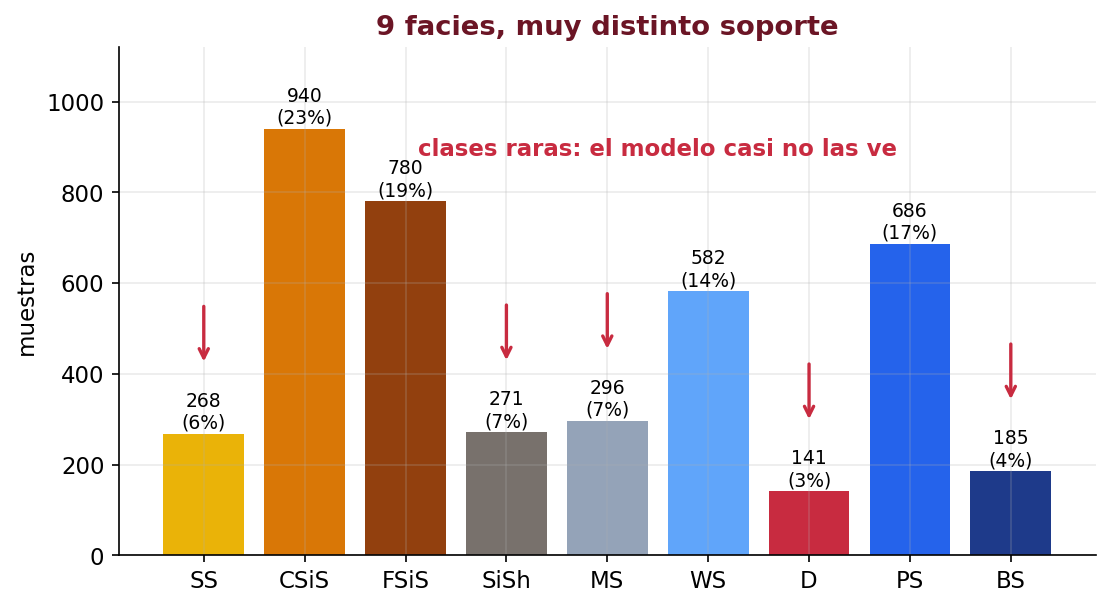
\includegraphics[width=\textwidth]{fig_balance.png}
    \end{column}
    \begin{column}{0.34\textwidth}
      {\footnotesize\color{textMuted}
      \begin{itemize}\setlength{\itemsep}{5pt}
        \item[{\color{arcaRed}\scriptsize\faArrowRight}]
          La limolita gruesa (\texttt{CSiS}) tiene \textbf{940} muestras;
          la dolomita (\texttt{D}), apenas \textbf{141}.
        \item[{\color{arcaRed}\scriptsize\faExclamationTriangle}]
          En la Clase 2 el desbalance era 2 a 1. Aquí es
          \textbf{7 a 1} entre la clase más común y la más rara.
        \item[{\color{arcaRed}\scriptsize\faBullseye}]
          Pregunta para dentro de un rato: ¿el modelo aprenderá
          la dolomita\ldots{} o la \textbf{ignorará}?
      \end{itemize}
      }
    \end{column}
  \end{columns}
\end{frame}

% ── GR POR FACIES ────────────────────────────────────────────────────────────
\begin{frame}{Explorar por Clase: el GR Cuenta una Historia}
  \vspace{-6pt}
  \begin{columns}[T]
    \begin{column}{0.62\textwidth}
      \centering
      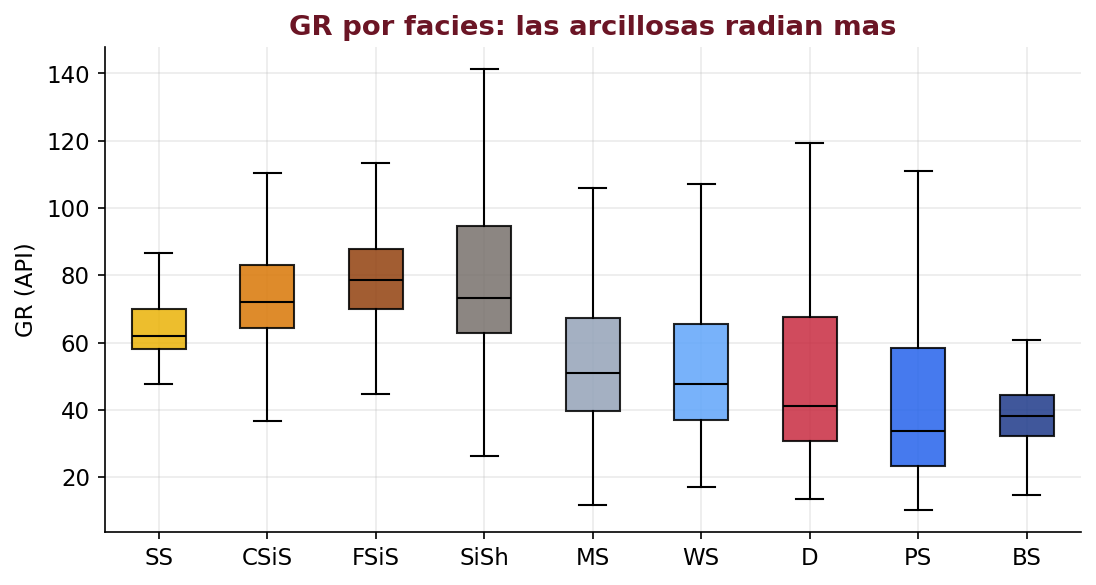
\includegraphics[width=\textwidth]{fig_box_gr.png}
    \end{column}
    \begin{column}{0.34\textwidth}
      {\footnotesize\color{textMuted}
      \begin{itemize}\setlength{\itemsep}{5pt}
        \item[{\color{codeGreen}\scriptsize\faCheck}]
          La física responde: las facies con más arcilla
          (\texttt{FSiS}, \texttt{SiSh}) \textbf{radian más};
          los carbonatos limpios (\texttt{PS}, \texttt{BS}), menos.
        \item[{\color{arcaRed}\scriptsize\faArrowRight}]
          Pero miren los \textbf{solapes}: con GR solo,
          \texttt{MS}, \texttt{WS} y \texttt{D} son casi indistinguibles.
        \item[{\color{arcaRed}\scriptsize\faBullseye}]
          Una variable no alcanza: necesitamos que el modelo
          \textbf{combine} las cinco curvas + el contexto.
      \end{itemize}
      }
    \end{column}
  \end{columns}
\end{frame}

% ── CROSSPLOT ────────────────────────────────────────────────────────────────
\begin{frame}{El Crossplot: por Esto Traemos al Bosque}
  \vspace{-6pt}
  \begin{columns}[T]
    \begin{column}{0.58\textwidth}
      \centering
      
\includegraphics[height=0.76\textheight]{fig_crossplot.png}
    \end{column}
    \begin{column}{0.38\textwidth}
      {\footnotesize\color{textMuted}
      \begin{itemize}\setlength{\itemsep}{5pt}
        \item[{\color{arcaRed}\scriptsize\faArrowRight}]
          9 nubes de puntos \textbf{encimadas}. No hay recta ---
          ni nueve rectas --- que las separen limpio.
        \item[{\color{codeGreen}\scriptsize\faCheck}]
          Es el mismo mensaje de las \textbf{lunas} de la Clase 3,
          pero con datos reales y 9 colores.
        \item[{\color{arcaRed}\scriptsize\faTree}]
          Por eso el modelo de hoy vuelve a ser el
          \textbf{Random Forest}: cortes no lineales,
          sin exigir escalado.
      \end{itemize}
      }
    \end{column}
  \end{columns}
\end{frame}

% ═════════════════════════════════════════════════════════════════════════════
\sectionframe{Codificar: el Idioma de los Modelos}{Los modelos solo comen números}
% ═════════════════════════════════════════════════════════════════════════════

% ── SOLO COMEN NÚMEROS ───────────────────────────────────────────────────────
\begin{frame}[shrink=8]{Los Modelos Solo Comen Números}
  \vspace{-4pt}
  {\small\color{arcaDark}\bfseries
    Todo lo que hay dentro de un modelo son sumas y comparaciones. ``Dolomita'' no se puede sumar.}

  \vspace{8pt}
  \begin{columns}[T]
    \begin{column}{0.48\textwidth}
      \begin{tcolorbox}[colback=arcaGray, colframe=arcaRed, boxrule=0pt, leftrule=3pt,
        arc=3pt, left=6pt, right=6pt, top=5pt, bottom=5pt]
        {\scriptsize\color{arcaRed}\bfseries\faKeyboard\hspace{4pt}USTEDES YA LO HACEN}\\[4pt]
        {\scriptsize\color{textMuted}
          Cuando llenan un formato de campo:
          ¿pozo fluyendo? \textbf{1}; ¿cerrado? \textbf{0}.
          ¿Tipo de levantamiento? marcan \textbf{una casilla}
          entre gas lift / BES / varilla.\\[3pt]
          Convertir categorías en casillas y unos-y-ceros
          es codificar. Solo falta ponerle nombre técnico.}
      \end{tcolorbox}
    \end{column}
    \begin{column}{0.48\textwidth}
      {\footnotesize\color{textMuted}
      \begin{itemize}\setlength{\itemsep}{5pt}
        \item[{\color{arcaRed}\scriptsize\faArrowRight}]
          En nuestra tabla hay \textbf{3 columnas de texto o categoría}:
          el target \texttt{Facies}, el contexto \texttt{NM\_M}
          y la \texttt{Formation}.
        \item[{\color{arcaRed}\scriptsize\faArrowRight}]
          Cada una necesita un \textbf{tratamiento distinto} ---
          y equivocarse de tratamiento \textbf{daña el modelo}
          en silencio.
        \item[{\color{codeGreen}\scriptsize\faCheck}]
          En 4 slides tendrán el \textbf{mapa completo}: qué técnica,
          para qué columna, y por qué.
      \end{itemize}
      }
    \end{column}
  \end{columns}
\end{frame}

% ── MAPA DE CODIFICACIÓN ─────────────────────────────────────────────────────
\begin{frame}[shrink=10]{El Mapa Completo de Codificación}
  \vspace{-4pt}
  {\small\color{arcaDark}\bfseries
    Tres técnicas. La pregunta clave es siempre: ¿cuántas categorías, y es target o feature?}

  \vspace{6pt}
  {\footnotesize
  \begin{tabular}{@{}lp{3.4cm}p{3.4cm}p{4.4cm}@{}}
    \toprule
    & {\color{arcaDark}\bfseries Binarizar} & {\color{arcaDark}\bfseries LabelEncoder}
      & {\color{arcaDark}\bfseries One-hot} \\
    \midrule
    Qué hace & 2 categorías \(\to\) 0 / 1 & N nombres \(\to\) 0\ldots N-1
      & 1 columna \(\to\) \textbf{N columnas} de 0/1 \\
    Se usa en & features de \textbf{2} valores & el \textbf{target} multiclase
      & features de \textbf{3+} valores \\
    Hoy & \texttt{NM\_M} \(\to\) \texttt{Marino} & \texttt{Facies} (9 nombres)
      & \texttt{Formation} (14 valores) \\
    Ya la vimos & Clase 2 (lutita 0/1) & hoy & hoy \\
    \bottomrule
  \end{tabular}
  }

  \vspace{8pt}
  {\footnotesize\color{textMuted}
  \begin{itemize}\setlength{\itemsep}{3pt}
    \item[{\color{arcaRed}\scriptsize\faExclamationTriangle}]
      ¿Por qué no usar LabelEncoder en una \textbf{feature} de 14 valores?
      Porque le inventa un \textbf{orden falso} a las categorías. Eso merece su propia slide.
    \item[{\color{arcaRed}\scriptsize\faExclamationTriangle}]
      ¿Y por qué no one-hot en el \textbf{target}? También lo veremos: error clásico.
  \end{itemize}
  }
\end{frame}

% ── TRAMPA ORDINAL ───────────────────────────────────────────────────────────
\begin{frame}[shrink=8]{La Trampa del Orden Falso}
  \vspace{-4pt}
  {\small\color{arcaDark}\bfseries
    Si numeramos arenisca = 1, caliza = 2, lutita = 3\ldots{} el modelo se lo cree.}

  \vspace{8pt}
  \centering
  \begin{tikzpicture}[scale=1.0]
    \draw[->, thick, textMuted] (0,0) -- (10.4,0);
    \node[below, font=\scriptsize\color{textMuted}] at (10.1,-0.08) {escala numérica};
    \foreach \x/\v in {1.5/1, 5.0/2, 8.5/3} {
      \draw[thick, textMuted] (\x,-0.09) -- (\x,0.09);
      \node[below, font=\scriptsize\bfseries\color{textDark}] at (\x,-0.15) {\v};
    }
    \node[above, font=\small\bfseries\color{facSS}] at (1.5,0.25) {arenisca};
    \node[above, font=\small\bfseries\color{facPS}] at (5.0,0.25) {caliza};
    \node[above, font=\small\bfseries\color{facSiSh}] at (8.5,0.25) {lutita};
    \draw[decorate, decoration={brace, amplitude=5pt}, arcaRed, thick]
      (1.6,0.85) -- (8.4,0.85);
    \node[above, font=\scriptsize\bfseries\color{arcaRed}, text width=7cm, align=center]
      at (5.0,1.15) {para el modelo, la caliza queda ``a mitad de camino''\\
        entre arenisca y lutita --- \textbf{geológicamente falso}};
  \end{tikzpicture}

  \vspace{10pt}
  {\footnotesize\color{textMuted}
  \begin{itemize}\setlength{\itemsep}{4pt}
    \item[{\color{arcaRed}\scriptsize\faArrowRight}]
      Los números traen \textbf{orden y distancia} de regalo: \(2\) está entre \(1\) y \(3\),
      y \(3-1=2\). Las categorías geológicas \textbf{no tienen} nada de eso.
    \item[{\color{arcaRed}\scriptsize\faExclamationTriangle}]
      Nuestro dataset ya viene con la trampa puesta: \texttt{Facies} llega como
      números 1--9. Por eso lo primero será \textbf{devolverles su nombre}.
  \end{itemize}
  }
\end{frame}

% ── PRUEBA: REGRESIÓN SOBRE EL NÚMERO ────────────────────────────────────────
\begin{frame}[fragile,shrink=22]{La Prueba: ¿y si Tratamos la Facies como Número?}
  \vspace{-4pt}
  {\small\color{arcaDark}\bfseries
    Hagamos el experimento del error: predecir el \emph{número} de facies con regresión.}

  \vspace{4pt}
  \begin{columns}[T]
    \begin{column}{0.54\textwidth}
      \begin{pyblock}
from sklearn.ensemble import RandomForestRegressor

reg = RandomForestRegressor(random_state=42)
reg.fit(X_tr, y_tr)
print(reg.predict(X_te)[:6].round(2))
      \end{pyblock}
      \vspace{2pt}
      \begin{outputblock}[]
[5.12 3.97 4.37 3.02 6.63 2.82]
      \end{outputblock}
    \end{column}
    \begin{column}{0.42\textwidth}
      {\scriptsize\color{textMuted}
      \begin{itemize}\setlength{\itemsep}{5pt}
        \item[{\color{arcaRed}\scriptsize\faTimes}]
          ¿Facies \textbf{4.37}? \textbf{No existe.} El modelo
          promedia categorías como si fueran barriles.
        \item[{\color{arcaRed}\scriptsize\faTimes}]
          Si redondeamos a la facies más cercana:
          accuracy \textbf{0.40}, contra \textbf{0.76}
          clasificando como se debe.
        \item[{\color{codeGreen}\scriptsize\faCheck}]
          Moraleja: número \(\neq\) cantidad.
          Cuando la variable es una \textbf{categoría},
          el problema es de \textbf{clasificación}. Siempre.
      \end{itemize}
      }
    \end{column}
  \end{columns}
\end{frame}

% ── LABELENCODER ─────────────────────────────────────────────────────────────
\begin{frame}[fragile,shrink=22]{LabelEncoder: el Diccionario del Target}
  \vspace{-4pt}
  {\small\color{arcaDark}\bfseries
    Para el \textbf{target} sí usamos números 0\ldots8 --- pero como \emph{código}, no como cantidad.}

  \vspace{4pt}
  \begin{columns}[T]
    \begin{column}{0.56\textwidth}
      \begin{pyblock}
from sklearn.preprocessing import LabelEncoder

le = LabelEncoder()
y = le.fit_transform(df['FaciesNombre'])
print(le.classes_)
print(y[:3], '->',
      le.inverse_transform(y[:3]))
      \end{pyblock}
      \vspace{2pt}
      \begin{outputblock}[]
['BS' 'CSiS' 'D' 'FSiS' 'MS' 'PS' 'SS'
 'SiSh' 'WS']
[3 3 3] -> ['FSiS' 'FSiS' 'FSiS']
      \end{outputblock}
    \end{column}
    \begin{column}{0.40\textwidth}
      {\scriptsize\color{textMuted}
      \begin{itemize}\setlength{\itemsep}{5pt}
        \item[{\color{arcaRed}\scriptsize\faBook}]
          Es un \textbf{diccionario de ida y vuelta}:
          \texttt{fit\_transform} pone códigos,
          \texttt{inverse\_transform} devuelve nombres.
        \item[{\color{codeGreen}\scriptsize\faCheck}]
          En el target no hay trampa ordinal: el clasificador
          trata cada código como \textbf{casilla separada},
          nunca hace cuentas con ellos.
        \item[{\color{arcaRed}\scriptsize\faArrowRight}]
          Regla: LabelEncoder \(\to\) \textbf{solo el target}.
          Para features categóricas, lo que sigue.
      \end{itemize}
      }
    \end{column}
  \end{columns}
\end{frame}

% ── ONE-HOT ──────────────────────────────────────────────────────────────────
\begin{frame}[fragile,shrink=22]{One-Hot: una Casilla por Categoría}
  \vspace{-4pt}
  {\small\color{arcaDark}\bfseries
    Para features categóricas: cada valor se vuelve su \textbf{propia columna} de 0/1. Sin orden, sin trampa.}

  \vspace{4pt}
  \begin{columns}[T]
    \begin{column}{0.56\textwidth}
      \begin{pyblock}
oh = pd.get_dummies(df['Formation'],
                    prefix='Fm')
print(oh.shape[1], 'columnas nuevas')
print(list(oh.columns[:3]))

df['Marino'] = (df['NM_M'] == 2).astype(int)
      \end{pyblock}
      \vspace{2pt}
      \begin{outputblock}
14 columnas nuevas
['Fm_A1 LM', 'Fm_A1 SH', 'Fm_B1 LM']
      \end{outputblock}
    \end{column}
    \begin{column}{0.40\textwidth}
      {\scriptsize\color{textMuted}
      \begin{itemize}\setlength{\itemsep}{5pt}
        \item[{\color{arcaRed}\scriptsize\faColumns}]
          \texttt{Formation} (14 valores) \(\to\) \textbf{14 columnas}.
          Cada fila tiene un solo 1: su casilla.
        \item[{\color{codeGreen}\scriptsize\faCheck}]
          \texttt{NM\_M} tiene solo 2 valores \(\to\) basta
          \textbf{binarizar}: \texttt{Marino} = 0/1,
          igual que la lutita de la Clase 2.
        \item[{\color{arcaRed}\scriptsize\faExclamationTriangle}]
          El precio del one-hot: \textbf{más columnas}.
          Con 14 valores va bien; con 10\,000 (un ID de pozo)
          sería una mala idea.
      \end{itemize}
      }
    \end{column}
  \end{columns}
\end{frame}

% ── ERROR CLÁSICO: ONE-HOT EN TARGET ─────────────────────────────────────────
\begin{frame}[shrink=8]{El Error Clásico: One-Hot en el Target}
  \vspace{-4pt}
  {\small\color{arcaDark}\bfseries
    ``Si one-hot es tan bueno\ldots{} ¿por qué no se lo aplico a \texttt{Facies}?''}

  \vspace{8pt}
  \begin{columns}[T]
    \begin{column}{0.48\textwidth}
      \begin{tcolorbox}[colback=arcaGray, colframe=arcaRed, boxrule=0pt, leftrule=3pt,
        arc=3pt, left=6pt, right=6pt, top=5pt, bottom=5pt]
        {\scriptsize\color{arcaRed}\bfseries\faTimes\hspace{4pt}LO QUE PASA SI LO HACEN}\\[4pt]
        {\scriptsize\color{textMuted}
          El target deja de ser una columna y se vuelve 9.
          \texttt{scikit-learn} cree que son \textbf{9 problemas
          independientes} de sí/no\ldots{} y puede responder
          ``sí'' a dos facies a la vez, o a ninguna.}
      \end{tcolorbox}
      \vspace{6pt}
      {\scriptsize\color{textMuted}\itshape
        Una muestra tiene \textbf{exactamente una} facies:
        el target debe ser \textbf{una sola columna} de códigos.}
    \end{column}
    \begin{column}{0.48\textwidth}
      {\footnotesize\color{textMuted}
      \begin{itemize}\setlength{\itemsep}{5pt}
        \item[{\color{codeGreen}\scriptsize\faCheck}]
          Regla de bolsillo, para pegar en el monitor:
        \item[{\color{arcaRed}\scriptsize\faArrowRight}]
          \textbf{Target} categórico \(\to\) \texttt{LabelEncoder}
          (una columna de códigos).
        \item[{\color{arcaRed}\scriptsize\faArrowRight}]
          \textbf{Feature} con 2 valores \(\to\) binarizar (0/1).
        \item[{\color{arcaRed}\scriptsize\faArrowRight}]
          \textbf{Feature} con 3+ valores \(\to\) one-hot
          (\texttt{get\_dummies}).
        \item[{\color{arcaRed}\scriptsize\faBan}]
          Números ordinales inventados en features \(\to\) \textbf{nunca},
          salvo que el orden sea real (p.\,ej.\ calidad mala/media/buena).
      \end{itemize}
      }
    \end{column}
  \end{columns}
\end{frame}

% ── CODIFICAR PAGA ───────────────────────────────────────────────────────────
\begin{frame}[shrink=10]{¿Y Todo Este Esfuerzo Paga?}
  \vspace{-4pt}
  {\small\color{arcaDark}\bfseries
    Midámoslo: mismo modelo, con y sin las columnas codificadas.}

  \vspace{8pt}
  \centering
  {\footnotesize
  \begin{tabular}{@{}lcc c@{}}
    \toprule
    {\color{arcaDark}\bfseries Modelo} &
    {\color{arcaDark}\bfseries Solo 6 registros} &
    {\color{arcaDark}\bfseries + \texttt{Marino} + one-hot} &
    {\color{arcaDark}\bfseries Ganancia} \\
    \midrule
    Logística multiclase & 0.511 & 0.594 & {\color{codeGreen}\bfseries +8.3 pts} \\
    Random Forest & 0.697 & \textbf{0.764} & {\color{codeGreen}\bfseries +6.7 pts} \\
    \bottomrule
  \end{tabular}
  }

  \vspace{12pt}
  {\footnotesize\color{textMuted}
  \begin{itemize}\setlength{\itemsep}{4pt}
    \item[{\color{codeGreen}\scriptsize\faCheck}]
      El \textbf{contexto geológico} (marino/no marino, formación) que ustedes
      darían por obvio, el modelo \textbf{no lo ve} hasta que se lo codifican.
    \item[{\color{arcaRed}\scriptsize\faArrowRight}]
      Codificar bien no es burocracia: son \textbf{6--8 puntos de accuracy gratis} ---
      más que muchos cambios de modelo.
  \end{itemize}
  }
\end{frame}

% ═════════════════════════════════════════════════════════════════════════════
\sectionframe{El Bosque, Ahora con 9 Clases}{El mismo código, un problema más grande}
% ═════════════════════════════════════════════════════════════════════════════

% ── RF EN CÓDIGO ─────────────────────────────────────────────────────────────
\begin{frame}[fragile,shrink=22]{Random Forest Multiclase: el Mismo Código de la Clase 3}
  \vspace{-4pt}
  {\small\color{arcaDark}\bfseries
    Prometido: el flujo no cambia. \texttt{scikit-learn} cuenta las clases de \texttt{y} y listo.}

  \vspace{4pt}
  \begin{columns}[T]
    \begin{column}{0.54\textwidth}
      \begin{pyblock}
from sklearn.ensemble import RandomForestClassifier

rf = RandomForestClassifier(
    n_estimators=200, random_state=42)
rf.fit(X_tr, y_tr)
print(round(rf.score(X_te, y_te), 3))
      \end{pyblock}
      \vspace{2pt}
      \begin{outputblock}
0.764
      \end{outputblock}
    \end{column}
    \begin{column}{0.42\textwidth}
      {\scriptsize\color{textMuted}
      \begin{itemize}\setlength{\itemsep}{5pt}
        \item[{\color{codeGreen}\scriptsize\faCheck}]
          \textbf{76.4\,\%} de aciertos exactos entre
          \textbf{9 opciones}. El azar puro daría 11\,\%;
          el modelo tonto, 23\,\%.
        \item[{\color{arcaRed}\scriptsize\faArrowRight}]
          Cada árbol vota por \textbf{una de las 9 facies};
          gana la mayoría. La misma democracia de la Clase 3.
        \item[{\color{arcaRed}\scriptsize\faEye}]
          ¿76\,\% es \emph{bueno}? Con accuracy sola
          \textbf{no se puede saber}. Necesitamos abrir la caja
          --- sección siguiente.
      \end{itemize}
      }
    \end{column}
  \end{columns}
\end{frame}

% ── MARCADOR ─────────────────────────────────────────────────────────────────
\begin{frame}[shrink=10]{El Marcador: Tres Modelos, Mismo Test}
  \vspace{-4pt}
  {\small\color{arcaDark}\bfseries
    Como siempre: cualquier modelo se compara contra el tonto y contra el lineal.}

  \vspace{8pt}
  \centering
  {\footnotesize
  \begin{tabular}{@{}lccc@{}}
    \toprule
    {\color{arcaDark}\bfseries Modelo} & {\color{arcaDark}\bfseries Accuracy} &
    {\color{arcaDark}\bfseries F1 macro} & {\color{arcaDark}\bfseries F1 weighted} \\
    \midrule
    Modelo tonto (siempre \texttt{CSiS}) & 0.229 & 0.041 & 0.085 \\
    Logística multiclase (escalada) & 0.594 & 0.573 & 0.592 \\
    \rowcolor{arcaGray}
    \textbf{Random Forest (200 árboles)} & \textbf{0.764} & \textbf{0.754} & \textbf{0.763} \\
    \bottomrule
  \end{tabular}
  }

  \vspace{12pt}
  {\footnotesize\color{textMuted}
  \begin{itemize}\setlength{\itemsep}{4pt}
    \item[{\color{codeGreen}\scriptsize\faCheck}]
      La \textbf{no linealidad} vuelve a pagar: +17 puntos sobre la recta,
      igual que nos pasó con las lunas y la litología en la Clase 3.
    \item[{\color{arcaRed}\scriptsize\faArrowRight}]
      Aparecieron dos columnas nuevas en el marcador: \textbf{F1 macro} y
      \textbf{F1 weighted}. Explicarlas --- y entender a quién protege cada una ---
      es el corazón de lo que sigue.
  \end{itemize}
  }
\end{frame}

% ═════════════════════════════════════════════════════════════════════════════
\sectionframe{Leer 9 Clases a la Vez}{La matriz de confusión ahora es \(9\times9\)}
% ═════════════════════════════════════════════════════════════════════════════

% ── MATRIZ 9x9 ───────────────────────────────────────────────────────────────
\begin{frame}{La Matriz de Confusión, Versión \(9\times9\)}
  \vspace{-6pt}
  \begin{columns}[T]
    \begin{column}{0.52\textwidth}
      \centering
      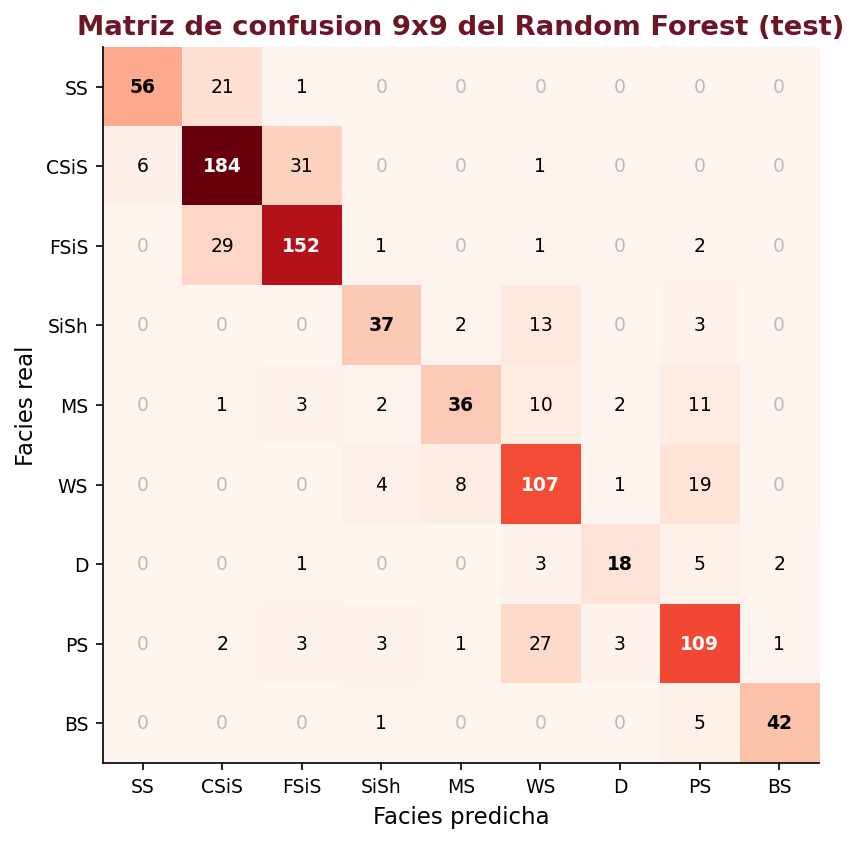
\includegraphics[height=0.78\textheight]{fig_confusion_rf.png}
    \end{column}
    \begin{column}{0.44\textwidth}
      {\footnotesize\color{textMuted}
      \begin{itemize}\setlength{\itemsep}{5pt}
        \item[{\color{arcaRed}\scriptsize\faArrowRight}]
          Se lee igual que la \(2\times2\) de la Clase 2:
          \textbf{fila = lo que era}, \textbf{columna = lo que dijo
          el modelo}. La diagonal son los aciertos.
        \item[{\color{codeGreen}\scriptsize\faCheck}]
          Ordenamos las facies \textbf{geológicamente}
          (no marinas primero, marinas después) y aparece algo:
          los errores se \textbf{pegan a la diagonal}.
        \item[{\color{arcaRed}\scriptsize\faEye}]
          Cada casilla fuera de la diagonal es una historia:
          ¿\emph{por qué} confundió 31 limolitas gruesas con finas?
        \item[{\color{arcaRed}\scriptsize\faBullseye}]
          Con 9 clases, esta matriz \textbf{es} el reporte del modelo.
          La accuracy es solo su resumen de una línea.
      \end{itemize}
      }
    \end{column}
  \end{columns}
\end{frame}

% ── LECTURA GEOLÓGICA ────────────────────────────────────────────────────────
\begin{frame}[shrink=10]{Leerla con Ojos de Geólogo}
  \vspace{-4pt}
  {\small\color{arcaDark}\bfseries
    Pregunta obligada: ¿los errores del modelo tienen sentido físico?}

  \vspace{6pt}
  \begin{columns}[T]
    \begin{column}{0.52\textwidth}
      {\footnotesize\color{textMuted}
      Las confusiones más frecuentes del bosque:}
      \vspace{2pt}
      {\footnotesize
      \begin{tabular}{@{}lcr@{}}
        \toprule
        {\color{arcaDark}\bfseries Real \(\to\) predicha} & {\color{arcaDark}\bfseries Casos}
          & {\color{arcaDark}\bfseries ¿Vecinas?} \\
        \midrule
        \texttt{CSiS} \(\to\) \texttt{FSiS} & 31 & {\color{codeGreen}\faCheck} \\
        \texttt{FSiS} \(\to\) \texttt{CSiS} & 29 & {\color{codeGreen}\faCheck} \\
        \texttt{PS} \(\to\) \texttt{WS} & 27 & {\color{codeGreen}\faCheck} \\
        \texttt{SS} \(\to\) \texttt{CSiS} & 21 & {\color{codeGreen}\faCheck} \\
        \texttt{WS} \(\to\) \texttt{PS} & 19 & {\color{codeGreen}\faCheck} \\
        \bottomrule
      \end{tabular}
      }
    \end{column}
    \begin{column}{0.44\textwidth}
      {\footnotesize\color{textMuted}
      \begin{itemize}\setlength{\itemsep}{5pt}
        \item[{\color{codeGreen}\scriptsize\faCheck}]
          El modelo confunde \textbf{limolita gruesa con fina} y
          \textbf{packstone con wackestone}: exactamente lo que
          confundiría un geólogo con el registro en la mano.
        \item[{\color{arcaRed}\scriptsize\faArrowRight}]
          De los 229 errores del bosque, \textbf{el 67\,\% cae en una
          facies geológicamente vecina}.
        \item[{\color{arcaRed}\scriptsize\faBullseye}]
          Un modelo que se equivoca ``con sentido'' inspira más
          confianza que uno que acierta más pero delira cuando falla.
      \end{itemize}
      }
    \end{column}
  \end{columns}
\end{frame}

% ── PRECISION/RECALL POR CLASE ───────────────────────────────────────────────
\begin{frame}[shrink=14]{Precision y Recall, Ahora por Clase}
  \vspace{-4pt}
  {\small\color{arcaDark}\bfseries
    Las definiciones de la Clase 2 no cambian --- solo que ahora hay un par por facies.}

  \vspace{4pt}
  \begin{columns}[T]
    \begin{column}{0.5\textwidth}
      {\footnotesize
      \begin{tabular}{@{}lrrrr@{}}
        \toprule
        {\color{arcaDark}\bfseries Facies} & {\color{arcaDark}\bfseries Soporte} &
        {\color{arcaDark}\bfseries Prec.} & {\color{arcaDark}\bfseries Recall} &
        {\color{arcaDark}\bfseries F1} \\
        \midrule
        \texttt{SS}   &  78 & 0.90 & 0.72 & 0.80 \\
        \texttt{CSiS} & 222 & 0.78 & 0.83 & 0.80 \\
        \texttt{FSiS} & 185 & 0.80 & 0.82 & 0.81 \\
        \texttt{SiSh} &  55 & 0.77 & 0.67 & 0.72 \\
        {\color{arcaRed}\texttt{MS}} & {\color{arcaRed}65} & {\color{arcaRed}0.77}
          & {\color{arcaRed}\bfseries 0.55} & {\color{arcaRed}0.64} \\
        \texttt{WS}   & 139 & 0.66 & 0.77 & 0.71 \\
        {\color{arcaRed}\texttt{D}} & {\color{arcaRed}29} & {\color{arcaRed}0.75}
          & {\color{arcaRed}\bfseries 0.62} & {\color{arcaRed}0.68} \\
        \texttt{PS}   & 149 & 0.71 & 0.73 & 0.72 \\
        \texttt{BS}   &  48 & 0.93 & 0.88 & 0.90 \\
        \bottomrule
      \end{tabular}
      }
    \end{column}
    \begin{column}{0.46\textwidth}
      {\scriptsize\color{textMuted}
      \begin{itemize}\setlength{\itemsep}{5pt}
        \item[{\color{arcaRed}\scriptsize\faArrowRight}]
          \textbf{Recall de \texttt{MS}} = de todos los mudstone reales,
          ¿qué fracción encontró? Solo el \textbf{55\,\%}.
        \item[{\color{arcaRed}\scriptsize\faArrowRight}]
          \textbf{Precision de \texttt{MS}} = cuando dice mudstone,
          ¿qué tan confiable es? El 77\,\%.
        \item[{\color{arcaRed}\scriptsize\faExclamationTriangle}]
          Las clases en rojo son las de \textbf{soporte chico}:
          el modelo las aprende peor. El desbalance de la
          exploración \textbf{ya está cobrando}.
        \item[{\color{codeGreen}\scriptsize\faCheck}]
          En \texttt{sklearn}, todo esto sale de una línea:
          \texttt{classification\_report()}.
      \end{itemize}
      }
    \end{column}
  \end{columns}
\end{frame}

% ── MODELO PEREZOSO ──────────────────────────────────────────────────────────
\begin{frame}{El Modelo Perezoso: la Ceguera a las Clases Raras}
  \vspace{-6pt}
  \begin{columns}[T]
    \begin{column}{0.62\textwidth}
      \centering
      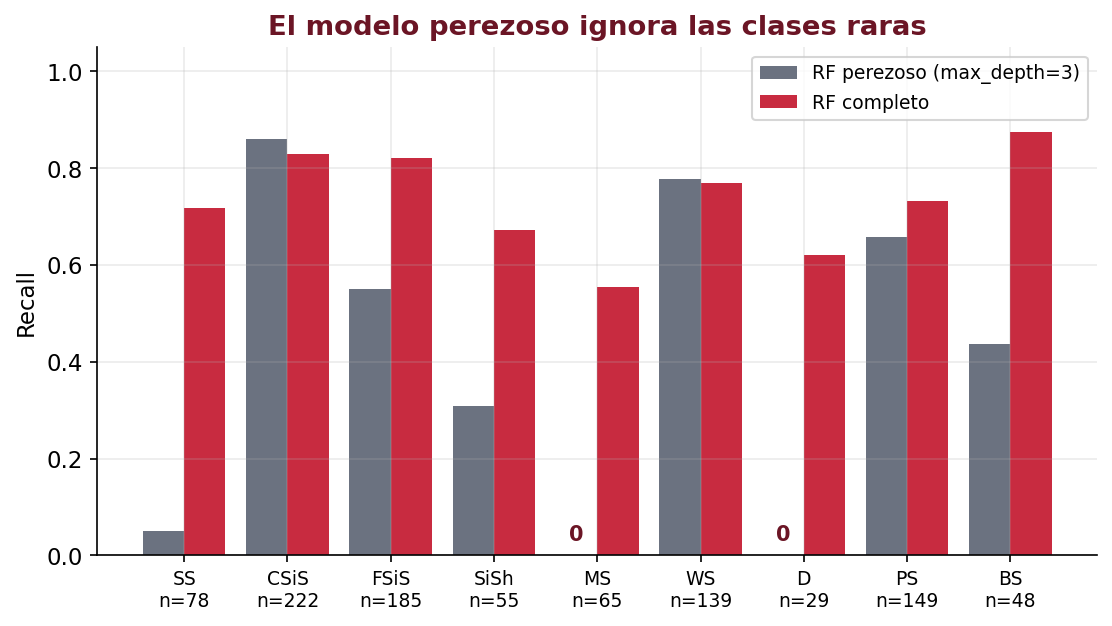
\includegraphics[width=\textwidth]{fig_recall_clases.png}
    \end{column}
    \begin{column}{0.34\textwidth}
      {\footnotesize\color{textMuted}
      \begin{itemize}\setlength{\itemsep}{5pt}
        \item[{\color{arcaRed}\scriptsize\faArrowRight}]
          Entrenamos a propósito un bosque \textbf{recortado}
          (\texttt{max\_depth=3}): accuracy \textbf{0.56} ---
          suena aceptable.
        \item[{\color{arcaRed}\scriptsize\faTimes}]
          Pero miren: mudstone y dolomita,
          \textbf{recall = 0.00}. Para el modelo,
          \textbf{no existen}.
        \item[{\color{arcaRed}\scriptsize\faExclamationTriangle}]
          Es la estrategia perezosa: apostar siempre a las
          clases grandes. La accuracy \textbf{lo premia};
          las clases raras \textbf{lo pagan}.
      \end{itemize}
      }
    \end{column}
  \end{columns}
\end{frame}

% ── MACRO VS WEIGHTED: CONCEPTO ──────────────────────────────────────────────
\begin{frame}[shrink=8]{Dos Maneras de Promediar 9 Notas}
  \vspace{-4pt}
  {\small\color{arcaDark}\bfseries
    Tenemos 9 valores de F1 --- uno por facies. ¿Cómo los resumimos en un solo número?}

  \vspace{8pt}
  \begin{columns}[T]
    \begin{column}{0.48\textwidth}
      \begin{tcolorbox}[colback=arcaGray, colframe=codeBlue, boxrule=0pt, leftrule=3pt,
        arc=3pt, left=6pt, right=6pt, top=5pt, bottom=5pt]
        {\scriptsize\color{codeBlue}\bfseries\faBalanceScale\hspace{4pt}WEIGHTED (ponderado)}\\[4pt]
        {\scriptsize\color{textMuted}
          Cada clase pesa según su \textbf{tamaño}: la nota de
          \texttt{CSiS} (222 muestras) manda; la de \texttt{D}
          (29) casi no cuenta.\\[3pt]
          \textbf{Protege a las clases grandes.} Se parece a la accuracy.}
      \end{tcolorbox}
    \end{column}
    \begin{column}{0.48\textwidth}
      \begin{tcolorbox}[colback=arcaGray, colframe=arcaRed, boxrule=0pt, leftrule=3pt,
        arc=3pt, left=6pt, right=6pt, top=5pt, bottom=5pt]
        {\scriptsize\color{arcaRed}\bfseries\faBalanceScale\hspace{4pt}MACRO (parejo)}\\[4pt]
        {\scriptsize\color{textMuted}
          Promedio simple: \textbf{cada clase vale igual},
          tenga 29 o 222 muestras. La dolomita opina
          con la misma voz que la limolita.\\[3pt]
          \textbf{Protege a las clases raras.}}
      \end{tcolorbox}
    \end{column}
  \end{columns}

  \vspace{10pt}
  {\footnotesize\color{textMuted}
  \begin{itemize}\setlength{\itemsep}{4pt}
    \item[{\color{arcaRed}\scriptsize\faCalculator}]
      Cuenta rápida con 2 clases: una grande (900 muestras, F1 = 0.90) y una rara
      (100 muestras, F1 = 0.10). Weighted = \(0.9\times0.90 + 0.1\times0.10 = \textbf{0.82}\).
      Macro = \((0.90+0.10)/2 = \textbf{0.50}\). \textbf{El mismo modelo.}
    \item[{\color{arcaRed}\scriptsize\faArrowRight}]
      ¿Cuál reportar? Depende de \textbf{qué les duele perder}. Si la clase rara es
      la que importa (la dolomita productora\ldots), macro.
  \end{itemize}
  }
\end{frame}

% ── MACRO VS WEIGHTED: FIGURA ────────────────────────────────────────────────
\begin{frame}{Mismo Modelo, Dos Veredictos}
  \vspace{-6pt}
  \begin{columns}[T]
    \begin{column}{0.62\textwidth}
      \centering
      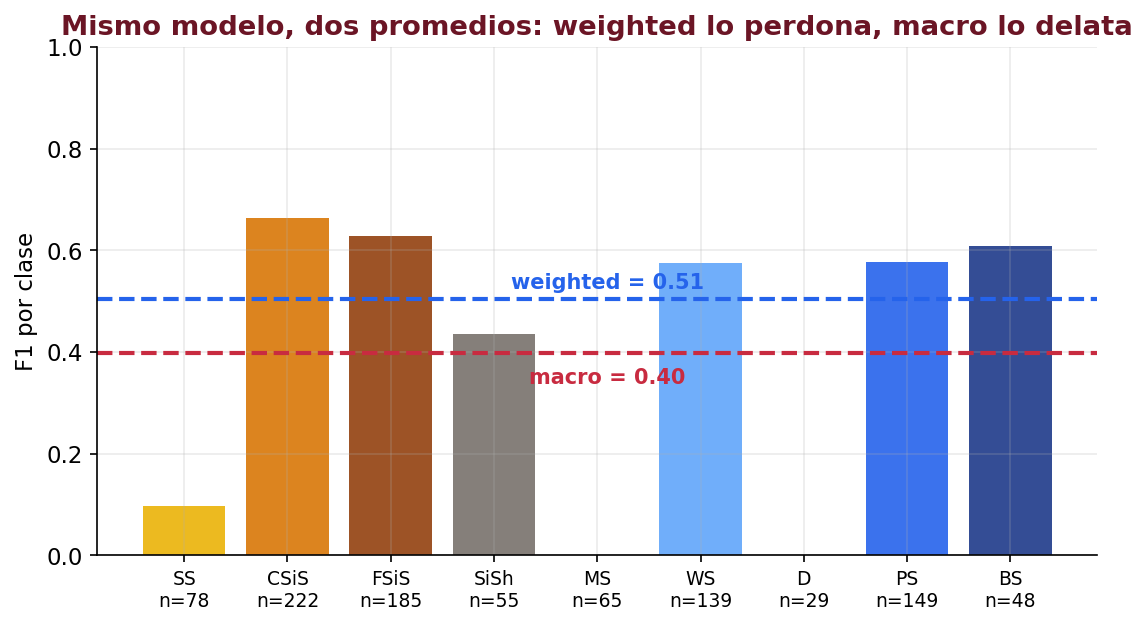
\includegraphics[width=\textwidth]{fig_macro_weighted.png}
    \end{column}
    \begin{column}{0.34\textwidth}
      {\footnotesize\color{textMuted}
      \begin{itemize}\setlength{\itemsep}{5pt}
        \item[{\color{arcaRed}\scriptsize\faArrowRight}]
          El modelo perezoso otra vez: F1 \textbf{weighted 0.51}
          (``regular''), F1 \textbf{macro 0.40} (``mal'').
        \item[{\color{arcaRed}\scriptsize\faEye}]
          La brecha entre los dos números es un \textbf{detector
          de clases abandonadas}: si macro \(\ll\) weighted,
          alguien quedó en cero.
        \item[{\color{codeGreen}\scriptsize\faCheck}]
          En nuestro bosque completo van parejas (0.754 vs 0.763):
          ninguna facies quedó abandonada del todo.
      \end{itemize}
      }
    \end{column}
  \end{columns}
\end{frame}

% ── PRÁCTICA 1 ───────────────────────────────────────────────────────────────
\begin{frame}[shrink=8]{Su Turno: la Logística Bajo la Lupa \hfill {\normalsize\color{arcaRed}\faClock\hspace{4pt}15 min}}
  \vspace{-4pt}
  {\small\color{arcaDark}\bfseries
    El bosque ya rindió cuentas clase por clase. Ahora háganle la misma auditoría a la logística.}

  \vspace{8pt}
  {\footnotesize
  \begin{enumerate}\setlength{\itemsep}{7pt}
    \item Entrenen la \textbf{logística multiclase} (con \texttt{StandardScaler},
      como en la Clase 2) sobre las mismas features codificadas.
    \item Saquen su \texttt{classification\_report}. ¿Qué facies tienen
      \textbf{recall} por debajo de 0.40?
    \item Comparen su \textbf{F1 macro} contra su \textbf{F1 weighted}.
      ¿La brecha delata clases abandonadas?
    \item Pregunta de negocio: si el cliente pregunta ``¿qué tan bueno es el
      modelo?'', ¿qué número le darían y \textbf{por qué ese}?
  \end{enumerate}
  }

  \vspace{8pt}
  {\scriptsize\color{textMuted}\itshape
    Pista: en el notebook está la celda lista con \texttt{\# Escribe tu solucion aqui}.}
\end{frame}

% ═════════════════════════════════════════════════════════════════════════════
\sectionframe{No Todos los Errores Cuestan Igual}{El costo de negocio, en 9 dimensiones}
% ═════════════════════════════════════════════════════════════════════════════

% ── MATRIZ DE PENALIZACIÓN ───────────────────────────────────────────────────
\begin{frame}[shrink=8]{La Matriz de Penalización}
  \vspace{-4pt}
  \begin{columns}[T]
    \begin{column}{0.5\textwidth}
      \centering
      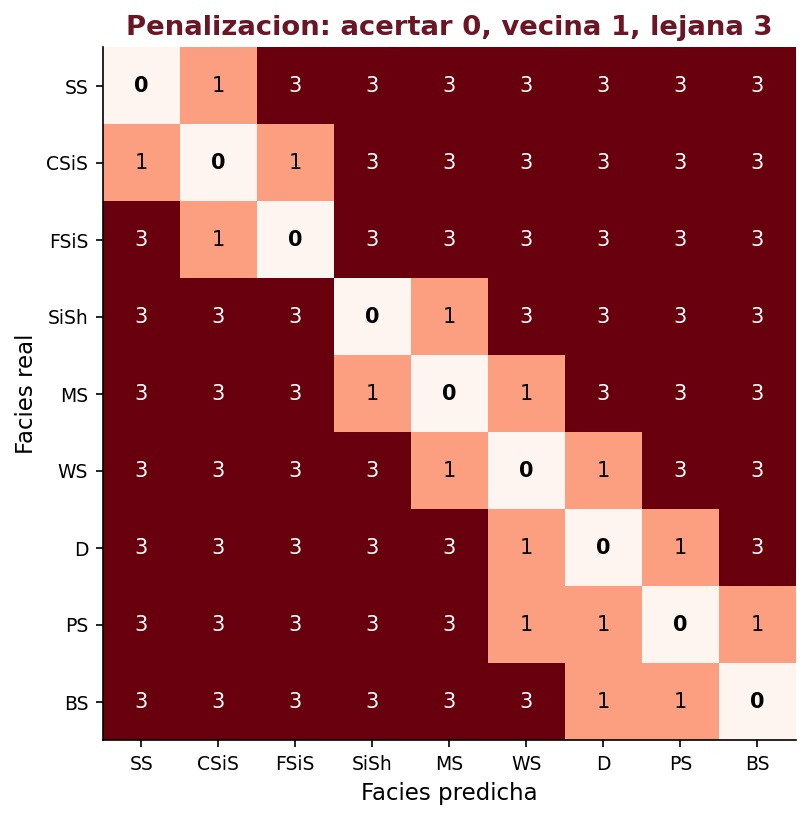
\includegraphics[height=0.74\textheight]{fig_penalizacion.png}
    \end{column}
    \begin{column}{0.46\textwidth}
      {\footnotesize\color{textMuted}
      \begin{itemize}\setlength{\itemsep}{5pt}
        \item[{\color{arcaRed}\scriptsize\faArrowRight}]
          En la Clase 2 el costo tenía 2 números (FP y FN).
          Con 9 clases necesita una \textbf{tabla completa}:
          cuánto duele confundir \emph{cada} facies con \emph{cada} otra.
        \item[{\color{codeGreen}\scriptsize\faCheck}]
          Nuestra regla, simple y geológica: acertar \textbf{0},
          facies \textbf{vecina 1} (limolita gruesa por fina: molesto),
          facies \textbf{lejana 3} (caliza por arenisca: grave).
        \item[{\color{arcaRed}\scriptsize\faTrophy}]
          No lo inventamos nosotros: la competencia SEG
          calificaba con una matriz así --- premiaba fallar cerca.
        \item[{\color{arcaRed}\scriptsize\faBullseye}]
          La matriz de penalización es la \textbf{traducción del
          negocio} al modelo: aquí es donde el ingeniero opina.
      \end{itemize}
      }
    \end{column}
  \end{columns}
\end{frame}

% ── RÉCORD ───────────────────────────────────────────────────────────────────
\begin{frame}{El Récord de Hoy: Penalización Total}
  \vspace{-6pt}
  \begin{columns}[T]
    \begin{column}{0.6\textwidth}
      \centering
      
\includegraphics[width=\textwidth]{fig_costo_modelos.png}
    \end{column}
    \begin{column}{0.36\textwidth}
      {\footnotesize\color{textMuted}
      \begin{itemize}\setlength{\itemsep}{5pt}
        \item[{\color{arcaRed}\scriptsize\faArrowRight}]
          Se calcula multiplicando \textbf{casilla por casilla}:
          matriz de confusión \(\times\) matriz de penalización,
          y sumando.
        \item[{\color{codeGreen}\scriptsize\faCheck}]
          El bosque no solo acierta más: \textbf{cuando falla,
          falla cerca}. Por eso su penalización cae a menos
          de la cuarta parte del tonto.
        \item[{\color{arcaRed}\scriptsize\faTrophy}]
          Récord del módulo, capítulo 3: en litología binaria
          fue 5\,953 \(\to\) 1\,150 (pesos); hoy es
          \textbf{1\,718 \(\to\) 379 puntos}.
      \end{itemize}
      }
    \end{column}
  \end{columns}
\end{frame}

% ── REPORTAR AL QUE DECIDE ───────────────────────────────────────────────────
\begin{frame}[shrink=16]{Cómo Reportarlo al que Decide}
  \vspace{-4pt}
  {\small\color{arcaDark}\bfseries
    El gerente no quiere oír ``F1 macro 0.754''. Quiere saber si puede confiar en el mapa de facies.}

  \vspace{8pt}
  \begin{columns}[T]
    \begin{column}{0.48\textwidth}
      \begin{tcolorbox}[colback=arcaGray, colframe=arcaRed, boxrule=0pt, leftrule=3pt,
        arc=3pt, left=6pt, right=6pt, top=5pt, bottom=5pt]
        {\scriptsize\color{arcaRed}\bfseries\faTimes\hspace{4pt}ASÍ NO}\\[4pt]
        {\scriptsize\color{textMuted}
          ``El clasificador alcanzó un accuracy de 0.764 con
          F1 macro de 0.754 y una penalización agregada de 379
          unidades sobre el conjunto de prueba.''}
      \end{tcolorbox}
      \vspace{6pt}
      \begin{tcolorbox}[colback=arcaGray, colframe=codeGreen, boxrule=0pt, leftrule=3pt,
        arc=3pt, left=6pt, right=6pt, top=5pt, bottom=5pt]
        {\scriptsize\color{codeGreen}\bfseries\faCheck\hspace{4pt}ASÍ SÍ}\\[4pt]
        {\scriptsize\color{textMuted}
          ``De cada 100 pies, el modelo acierta la facies exacta
          en \textbf{76} y en \textbf{92} queda a lo sumo en la
          vecina. Falla sobre todo entre limolitas --- el mismo
          punto ciego de un intérprete con solo registros.''}
      \end{tcolorbox}
    \end{column}
    \begin{column}{0.48\textwidth}
      {\footnotesize\color{textMuted}
      \begin{itemize}\setlength{\itemsep}{5pt}
        \item[{\color{arcaRed}\scriptsize\faArrowRight}]
          El número \textbf{92 de cada 100} sale de contar como
          aceptable la facies vecina: accuracy 0.764 exacta,
          \textbf{0.923} relajada.
        \item[{\color{arcaRed}\scriptsize\faArrowRight}]
          Digan también \textbf{dónde no confiar}: mudstone y
          dolomita (poco soporte, recall 0.55--0.62)
          ameritan revisión humana.
        \item[{\color{codeGreen}\scriptsize\faCheck}]
          Esto es lo que separa al ingeniero del que solo corre
          \texttt{.fit()}: traducir métricas a \textbf{decisiones
          con límites claros}.
      \end{itemize}
      }
    \end{column}
  \end{columns}
\end{frame}

% ── IMPORTANCIAS ─────────────────────────────────────────────────────────────
\begin{frame}{¿Qué Miró el Bosque para Lograrlo?}
  \vspace{-6pt}
  \begin{columns}[T]
    \begin{column}{0.6\textwidth}
      \centering
      
\includegraphics[width=\textwidth]{fig_importancia.png}
    \end{column}
    \begin{column}{0.36\textwidth}
      {\footnotesize\color{textMuted}
      \begin{itemize}\setlength{\itemsep}{5pt}
        \item[{\color{codeGreen}\scriptsize\faCheck}]
          Los \textbf{5 registros} dominan --- y \texttt{PE},
          el que casi botamos por sus faltantes, es el
          \textbf{segundo} más usado.
        \item[{\color{arcaRed}\scriptsize\faArrowRight}]
          Las columnas codificadas (\texttt{Marino}, one-hot de
          \texttt{Formation}) aportan menos por separado\ldots{}
          pero ya vimos que en conjunto valen \textbf{+6.7 puntos}.
        \item[{\color{arcaRed}\scriptsize\faExclamationTriangle}]
          Recordatorio de la Clase 3: importancia \(\neq\)
          causalidad. Es \emph{uso}, no física.
      \end{itemize}
      }
    \end{column}
  \end{columns}
\end{frame}

% ═════════════════════════════════════════════════════════════════════════════
\sectionframe{Las Perillas del Modelo}{Parámetros vs hiperparámetros}
% ═════════════════════════════════════════════════════════════════════════════

% ── PARAMS VS HIPERPARAMS ────────────────────────────────────────────────────
\begin{frame}[shrink=8]{Dos Tipos de Números Viven en un Modelo}
  \vspace{-4pt}
  {\small\color{arcaDark}\bfseries
    Ya usamos \texttt{max\_depth} y \texttt{n\_estimators} varias veces. Pongámosles apellido.}

  \vspace{8pt}
  \begin{columns}[T]
    \begin{column}{0.48\textwidth}
      \begin{tcolorbox}[colback=arcaGray, colframe=codeGreen, boxrule=0pt, leftrule=3pt,
        arc=3pt, left=6pt, right=6pt, top=5pt, bottom=5pt]
        {\scriptsize\color{codeGreen}\bfseries\faCogs\hspace{4pt}PARÁMETROS}\\[4pt]
        {\scriptsize\color{textMuted}
          Los aprende \textbf{el modelo solo}, desde los datos,
          durante \texttt{.fit()}.\\[3pt]
          Ejemplos: los \textbf{cortes} de cada árbol
          (``¿GR \(>\) 78?''), los coeficientes de la logística.\\[3pt]
          Ustedes \textbf{nunca los escriben}.}
      \end{tcolorbox}
    \end{column}
    \begin{column}{0.48\textwidth}
      \begin{tcolorbox}[colback=arcaGray, colframe=arcaRed, boxrule=0pt, leftrule=3pt,
        arc=3pt, left=6pt, right=6pt, top=5pt, bottom=5pt]
        {\scriptsize\color{arcaRed}\bfseries\faSlidersH\hspace{4pt}HIPERPARÁMETROS}\\[4pt]
        {\scriptsize\color{textMuted}
          Los eligen \textbf{ustedes}, \emph{antes} de entrenar.\\[3pt]
          Ejemplos: \texttt{max\_depth}, \texttt{n\_estimators},
          el \texttt{test\_size} del split.\\[3pt]
          Son las \textbf{perillas} del tablero: el modelo no puede
          girarlas por sí mismo.}
      \end{tcolorbox}
    \end{column}
  \end{columns}

  \vspace{10pt}
  {\footnotesize\color{textMuted}
  \begin{itemize}\setlength{\itemsep}{3pt}
    \item[{\color{arcaRed}\scriptsize\faArrowRight}]
      Analogía de taladro: el \textbf{peso sobre la broca} lo ajusta el perforador
      (perilla); el \textbf{desgaste} que va tomando la broca lo pone la formación
      (aprendido). Uno se decide, el otro resulta.
  \end{itemize}
  }
\end{frame}

% ── PERILLAS A MANO ──────────────────────────────────────────────────────────
\begin{frame}{Girando las Perillas a Mano}
  \vspace{-6pt}
  \begin{columns}[T]
    \begin{column}{0.64\textwidth}
      \centering
      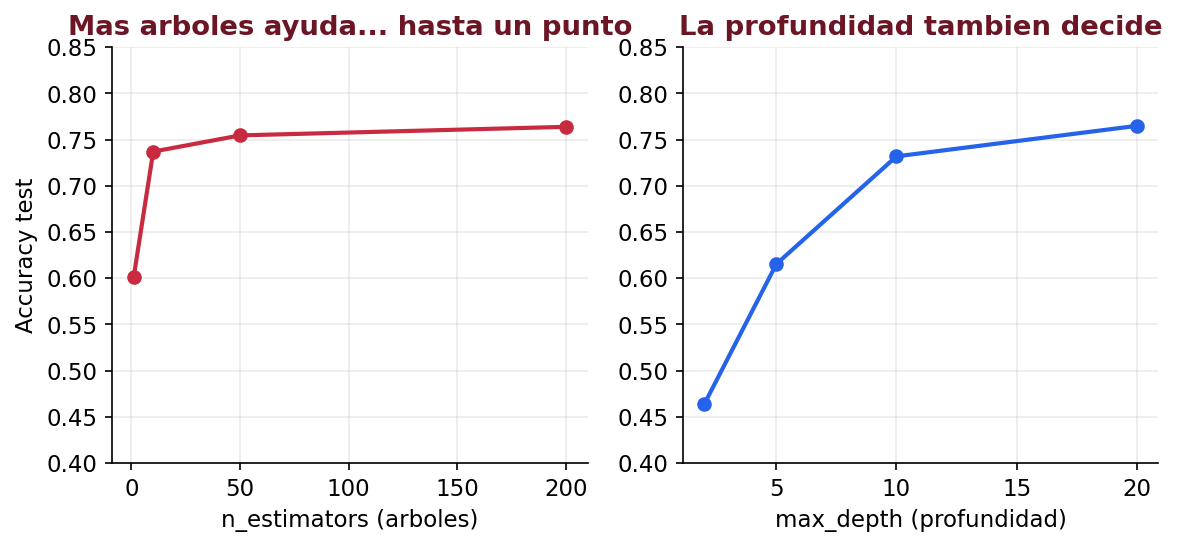
\includegraphics[width=\textwidth]{fig_hiperparams.png}
    \end{column}
    \begin{column}{0.32\textwidth}
      {\footnotesize\color{textMuted}
      \begin{itemize}\setlength{\itemsep}{5pt}
        \item[{\color{arcaRed}\scriptsize\faArrowRight}]
          Con 10 árboles ya casi todo está ganado;
          de 50 a 200 se rasca \textbf{un punto}.
        \item[{\color{arcaRed}\scriptsize\faArrowRight}]
          \texttt{max\_depth} recortado \textbf{cuesta caro}
          (ya vimos al perezoso).
        \item[{\color{arcaRed}\scriptsize\faQuestionCircle}]
          Pregunta incómoda: aquí elegimos perillas
          \textbf{mirando el test}\ldots{}
          ¿no es eso \textbf{hacer trampa}?
      \end{itemize}
      }
      \vspace{4pt}
      {\scriptsize\color{arcaDark}\itshape
        Sí lo es. La herramienta que lo hace bien
        viene en la siguiente slide.}
    \end{column}
  \end{columns}
\end{frame}

% ── GRIDSEARCH: CÓDIGO ───────────────────────────────────────────────────────
\begin{frame}[fragile,shrink=26]{GridSearchCV: la Búsqueda Automática de Perillas}
  \vspace{-4pt}
  {\small\color{arcaDark}\bfseries
    Le damos la \textbf{parrilla} de valores; él prueba todas las combinaciones --- sin tocar el test.}

  \vspace{4pt}
  \begin{columns}[T]
    \begin{column}{0.56\textwidth}
      \begin{pyblock}
from sklearn.model_selection import GridSearchCV

parrilla = {'max_depth': [5, 10, 20, None],
            'n_estimators': [50, 200]}
grid = GridSearchCV(
    RandomForestClassifier(random_state=42),
    parrilla, cv=5)
grid.fit(X_tr, y_tr)
print('mejor:', grid.best_params_)
      \end{pyblock}
      \vspace{2pt}
      \begin{outputblock}
mejor: {'max_depth': None,
        'n_estimators': 50}
      \end{outputblock}
    \end{column}
    \begin{column}{0.40\textwidth}
      {\scriptsize\color{textMuted}
      \begin{itemize}\setlength{\itemsep}{5pt}
        \item[{\color{arcaRed}\scriptsize\faTable}]
          \emph{Grid} = parrilla: \(4\times2 = \textbf{8}\)
          combinaciones de perillas.
        \item[{\color{arcaRed}\scriptsize\faRedo}]
          \texttt{cv=5}: cada combinación se valida \textbf{5 veces
          dentro del train} (por eso el test queda intacto).
          Son \(8\times5 = 40\) entrenamientos\ldots{} hechos por él.
        \item[{\color{codeGreen}\scriptsize\faCheck}]
          \texttt{best\_params\_}: la combinación ganadora.
          \texttt{best\_score\_}: su accuracy \textbf{de validación}
          (no de test).
      \end{itemize}
      }
    \end{column}
  \end{columns}
\end{frame}

% ── GRIDSEARCH: LECTURA ──────────────────────────────────────────────────────
\begin{frame}[shrink=10]{Qué Nos Dijo la Búsqueda}
  \vspace{-4pt}
  {\small\color{arcaDark}\bfseries
    La parrilla completa, con su accuracy de validación (promedio de los 5 pliegues).}

  \vspace{6pt}
  \begin{columns}[T]
    \begin{column}{0.46\textwidth}
      {\footnotesize
      \begin{tabular}{@{}ccc@{}}
        \toprule
        {\color{arcaDark}\bfseries max\_depth} & {\color{arcaDark}\bfseries n\_estimators}
          & {\color{arcaDark}\bfseries Validación} \\
        \midrule
        5 & 50 & 0.614 \\
        5 & 200 & 0.622 \\
        10 & 50 & 0.707 \\
        10 & 200 & 0.711 \\
        20 & 50 & 0.746 \\
        20 & 200 & 0.755 \\
        \rowcolor{arcaGray}
        \textbf{None} & \textbf{50} & \textbf{0.755} \\
        None & 200 & 0.748 \\
        \bottomrule
      \end{tabular}
      }
    \end{column}
    \begin{column}{0.5\textwidth}
      {\scriptsize\color{textMuted}
      \begin{itemize}\setlength{\itemsep}{5pt}
        \item[{\color{arcaRed}\scriptsize\faArrowRight}]
          La \textbf{profundidad} manda: de 5 a 20 niveles se ganan
          14 puntos. Los árboles (50 vs 200) mueven \textbf{décimas}.
        \item[{\color{arcaRed}\scriptsize\faEye}]
          Los dos primeros lugares empatan (0.755): a partir de
          cierta profundidad, \textbf{todo da más o menos igual}.
        \item[{\color{codeGreen}\scriptsize\faCheck}]
          El ganador en test: \textbf{0.755} --- prácticamente
          nuestro 0.764 de siempre. Moraleja honesta: \textbf{no siempre
          hay tesoro escondido}; la búsqueda sirve para \emph{confirmarlo
          sin hacer trampa}.
        \item[{\color{arcaRed}\scriptsize\faQuestionCircle}]
          ¿Por qué 5 pliegues? ¿Por qué funciona validar dentro del
          train? Eso \textbf{es} la Clase 5.
      \end{itemize}
      }
    \end{column}
  \end{columns}
\end{frame}

% ── PRÁCTICA 2 ───────────────────────────────────────────────────────────────
\begin{frame}[shrink=8]{Su Turno: su Propia Matriz de Penalización \hfill {\normalsize\color{arcaRed}\faClock\hspace{4pt}15 min}}
  \vspace{-4pt}
  {\small\color{arcaDark}\bfseries
    Nuestra matriz (0/1/3) es geológica. Háganla de negocio.}

  \vspace{8pt}
  {\footnotesize
  \begin{enumerate}\setlength{\itemsep}{7pt}
    \item Supongan que las facies de \textbf{buena roca almacén} son
      \texttt{SS}, \texttt{PS} y \texttt{BS}. Construyan una matriz donde
      confundir roca almacén con roca sello (o al revés) cueste \textbf{5},
      y cualquier otro error cueste \textbf{1}.
    \item Calculen la \textbf{penalización total} del Random Forest y de la
      logística con \emph{su} matriz. ¿Cambia el ganador?
    \item Encuentren en la matriz de confusión \textbf{la casilla que más plata
      les cuesta} con su regla. ¿Entre qué facies está?
    \item Pregunta de negocio: escriban \textbf{una frase para el gerente} de
      activos recomendando (o no) usar el modelo para mapear roca almacén.
    \item \textbf{Bonus} --- con \texttt{GridSearchCV}, agreguen
      \texttt{min\_samples\_leaf} \(\in \{1, 5, 20\}\) a la parrilla.
      ¿Cambia el ganador?
  \end{enumerate}
  }
\end{frame}

% ═════════════════════════════════════════════════════════════════════════════
\sectionframe{Cierre}{Lo que se llevan hoy}
% ═════════════════════════════════════════════════════════════════════════════

% ── RESUMEN ──────────────────────────────────────────────────────────────────
\begin{frame}[shrink=8]{Lo Que Aprendimos Hoy}
  \vspace{-4pt}
  \begin{columns}[T]
    \begin{column}{0.48\textwidth}
      {\footnotesize\color{arcaDark}\bfseries Conceptos}
      \vspace{3pt}
      {\footnotesize\color{textMuted}
      \begin{itemize}\setlength{\itemsep}{2pt}
        \item[{\color{codeGreen}\scriptsize\faCheck}]
          Multiclase: elegir una entre N (9 facies)
        \item[{\color{codeGreen}\scriptsize\faCheck}]
          Faltantes e imputación: el menú y cómo elegir
          según la \textbf{distribución}
        \item[{\color{codeGreen}\scriptsize\faCheck}]
          Codificar: binarizar / LabelEncoder / one-hot ---
          y cuándo usar cada una
        \item[{\color{codeGreen}\scriptsize\faCheck}]
          La trampa del orden falso (facies 4.37 no existe)
        \item[{\color{codeGreen}\scriptsize\faCheck}]
          Matriz \(9\times9\) leída \textbf{geológicamente}
        \item[{\color{codeGreen}\scriptsize\faCheck}]
          Macro vs weighted: a quién protege cada promedio
        \item[{\color{codeGreen}\scriptsize\faCheck}]
          Matriz de penalización: el costo en 9 dimensiones
        \item[{\color{codeGreen}\scriptsize\faCheck}]
          Parámetros vs hiperparámetros (las perillas)
      \end{itemize}
      }
    \end{column}
    \begin{column}{0.48\textwidth}
      {\footnotesize\color{arcaDark}\bfseries Herramientas}
      \vspace{3pt}
      {\footnotesize\color{textMuted}
      \begin{itemize}\setlength{\itemsep}{2pt}
        \item[{\color{arcaRed}\scriptsize\faTools}]
          \texttt{LabelEncoder} (+ \texttt{inverse\_transform})
        \item[{\color{arcaRed}\scriptsize\faTools}]
          \texttt{pd.get\_dummies} (one-hot)
        \item[{\color{arcaRed}\scriptsize\faTools}]
          \texttt{classification\_report}, \texttt{confusion\_matrix}
        \item[{\color{arcaRed}\scriptsize\faTools}]
          \texttt{f1\_score(average='macro' / 'weighted')}
        \item[{\color{arcaRed}\scriptsize\faTools}]
          \texttt{fillna} (mediana), \texttt{GridSearchCV}
      \end{itemize}
      }
      \vspace{8pt}
      \begin{tcolorbox}[colback=arcaGray, colframe=arcaRed, boxrule=0pt, leftrule=3pt,
        arc=3pt, left=6pt, right=6pt, top=5pt, bottom=5pt]
        {\scriptsize\color{arcaDark}\bfseries El número del día:}\\[3pt]
        {\scriptsize\color{textMuted}
          76 de 100 pies con la facies \textbf{exacta};
          92 de 100 a lo sumo en la \textbf{vecina}.
          Penalización: tonto \textbf{1\,718} \(\to\) bosque
          \textbf{379}.}
      \end{tcolorbox}
    \end{column}
  \end{columns}
\end{frame}

% ── PRÓXIMA ──────────────────────────────────────────────────────────────────
\begin{frame}{Lo Que Sigue: el Cierre del Módulo}
  \vspace{-6pt}
  {\small\color{arcaDark}\bfseries
    Clase 5: un modelo nuevo con una idea hermosa, y la respuesta a la pregunta incómoda.}

  \vspace{10pt}
  {\footnotesize
  \begin{itemize}\setlength{\itemsep}{7pt}
    \item[{\color{arcaRed}\Large\faArrowCircleRight}]
      \textbf{SVM y el truco del kernel} --- separar lo inseparable subiendo de
      dimensión (las lunas de la Clase 3 vuelven por última vez).

    \item[{\color{arcaRed}\Large\faArrowCircleRight}]
      \textbf{El porqué de la validación cruzada} --- hoy usamos
      \texttt{GridSearchCV} como receta; en la Clase 5 abrimos el \texttt{cv=5}
      y entendemos por qué protege del sobreajuste de perillas.

    \item[{\color{arcaRed}\Large\faArrowCircleRight}]
      \textbf{La deuda pendiente} --- validar con \textbf{pozos completos por fuera}:
      la anotamos en la Clase 2 y en la 3; en la 5 por fin se paga.
  \end{itemize}
  }

  \vspace{10pt}
  \centering
  {\footnotesize\color{arcaDark}\itshape
    Llegan a la Clase 5 sabiendo entrenar, codificar, evaluar y costear.
    Falta aprender a \textbf{afinar y validar como profesionales}.}
\end{frame}

% ── GRACIAS ──────────────────────────────────────────────────────────────────
\begingroup
\setbeamertemplate{headline}{}
\setbeamertemplate{footline}{}
\setbeamertemplate{navigation symbols}{}
\begin{frame}[plain, noframenumbering]
  \begin{tikzpicture}[remember picture, overlay]
    \fill[arcaDark] (current page.south west) rectangle (current page.north east);
    \node[anchor=center, text=white, font=\Huge\bfseries]
      at ([yshift=1.5cm]current page.center) {¡Gracias!};
    \node[anchor=center, text=white!80, font=\large, text width=10cm, align=center]
      at ([yshift=0.2cm]current page.center)
      {Carlos Enrique Mosquera Trujillo};
    \node[anchor=center, text=white!60, font=\normalsize, text width=10cm, align=center]
      at ([yshift=-0.6cm]current page.center)
      {\faEnvelope\hspace{6pt}cmosquerat@unal.edu.co};
    \node[anchor=center, text=white!60, font=\normalsize, text width=11cm, align=center]
      at ([yshift=-1.3cm]current page.center)
      {Machine Learning for Petroleum Engineers Using Python};
    \node[anchor=center, text=white!40, font=\small]
      at ([yshift=-2.0cm]current page.center)
      {SLB Ecuador \quad$\cdot$\quad UDLA \quad$\cdot$\quad 2026};
  \end{tikzpicture}
\end{frame}
\endgroup

\end{document}
